\chapter{Evaluation}
This chapter presents the evaluation of the implemented Moving Target Defense (MTD) framework with its techniques based on different criteria. First, the methodology of the evaluation is explained, followed by the missing prerequisites for the evaluation to work. The chapter then presents the evaluation process and its results. These results are discussed in Chapter \ref{chapter:discussion}.


\section{Evaluation Methodology} \label{section:evaluationMethodology}
The evaluation of the solution was quite complex because the whole setup had so many parts/scripts distributed across three different VMs. Ultimately, three different metrics were to be evaluated. The first and main evaluation metric is the total number of seconds that the two machines in the network are infected. This is reasonable as the goal of this thesis is to mitigate/prevent the infection of IoT devices and to show that a collaborative approach yields better results than a non-collaborative one. Thus, the fewer seconds the malware is running on the devices, the better. The other two metrics are defender metrics mentioned by~\cite{article:surveyMTD}, who investigated MTD research trends. Both metrics fall into the system performance category. 

The first system performance metric is the amount of time that incoming and outgoing communication to and from the device is interrupted. This can be further divided into the interruption caused by the IP address change and the interruption caused by the Telnet service port change. For the IP address change, only the outgoing connection was tested. The reason for this is that the incoming connection would only work if there was a mechanism to keep track of which machine has which IP address, similar to the one suggested by~\cite{NavasDefenseFramework}. However, outgoing connections are more critical, as IoT devices often need to pass on collected data. Regarding the Telnet service port change, incoming and outgoing connections to and from the Telnet port were evaluated. The other system performance metric is the CPU/RAM usage of the deployed MTD techniques, which is essential due to the hardware limitations of IoT devices.


Other potentially important metrics~\cite{article:surveyMTD} such as Quality of Service (QoS) to users or strategy switching costs were not included. This exclusion is due to the fact that these metrics were either out of scope or not feasible (e.g. power consumption). The three measured metrics were therefore:
\begin{enumerate}
    \item Total number of seconds that the machines are infected 
    \item Interruption of network availability of the machines
    \item CPU/RAM usage of the framework and the executing MTD techniques

\end{enumerate}

These metrics were measured in three different environments/systems for comparison. All environments used the VM structure already described, but differed in the solution applied and their deployment strategy (i.e. proactive vs. reactive deployment of MTD techniques). Environment 1 used a reactive, modified solution that did not include a cooperative component. This was done by only enabling the IP address change of infected machines. This approach already exists~\cite{article:vonderAssen}, but the implementation code of the approaches are independent. This environment allowed the collection of data from a solution that uses a non-cooperative and reactive defence approach, and served as a baseline for this evaluation. 

In contrast, Environment 2 used the IP address and the port change to reactively mitigate/prevent Bashlite. This environment allowed to collect data from a solution that uses a cooperative and reactive approach. Environment 3 used the cooperative approach (IP address change and Telnet service port change), but executed this proactively rather than reactively. This provided an interesting insight into the trade-offs/differences between the proactive and reactive approaches. While the reactive approaches were executed 10 seconds after Bashlite was executed, the proactive MTD techniques were executed every 60 seconds, regardless of whether Bashlite was active or not. The 60 seconds were initially chosen randomly, but proved to be a reasonable value given the results. Furthermore, the goal was to show the typical differences between the reactive and proactive approaches, rather than to determine an optimal time to move, as this would be influenced by many more factors of the system. Table \ref{graphic:tableEvaluationEnvironment} summarises the three environments.

The data was collected over 30 runs (entire infection/mitigation process) in each environment and is presented in Section \ref{section:results}. The first five of these 30 runs were removed from the data as they were used to warm up the entire system. Section 
\ref{section:gatheringData} describes the data collection in more detail. 


\begin{table}[tph]
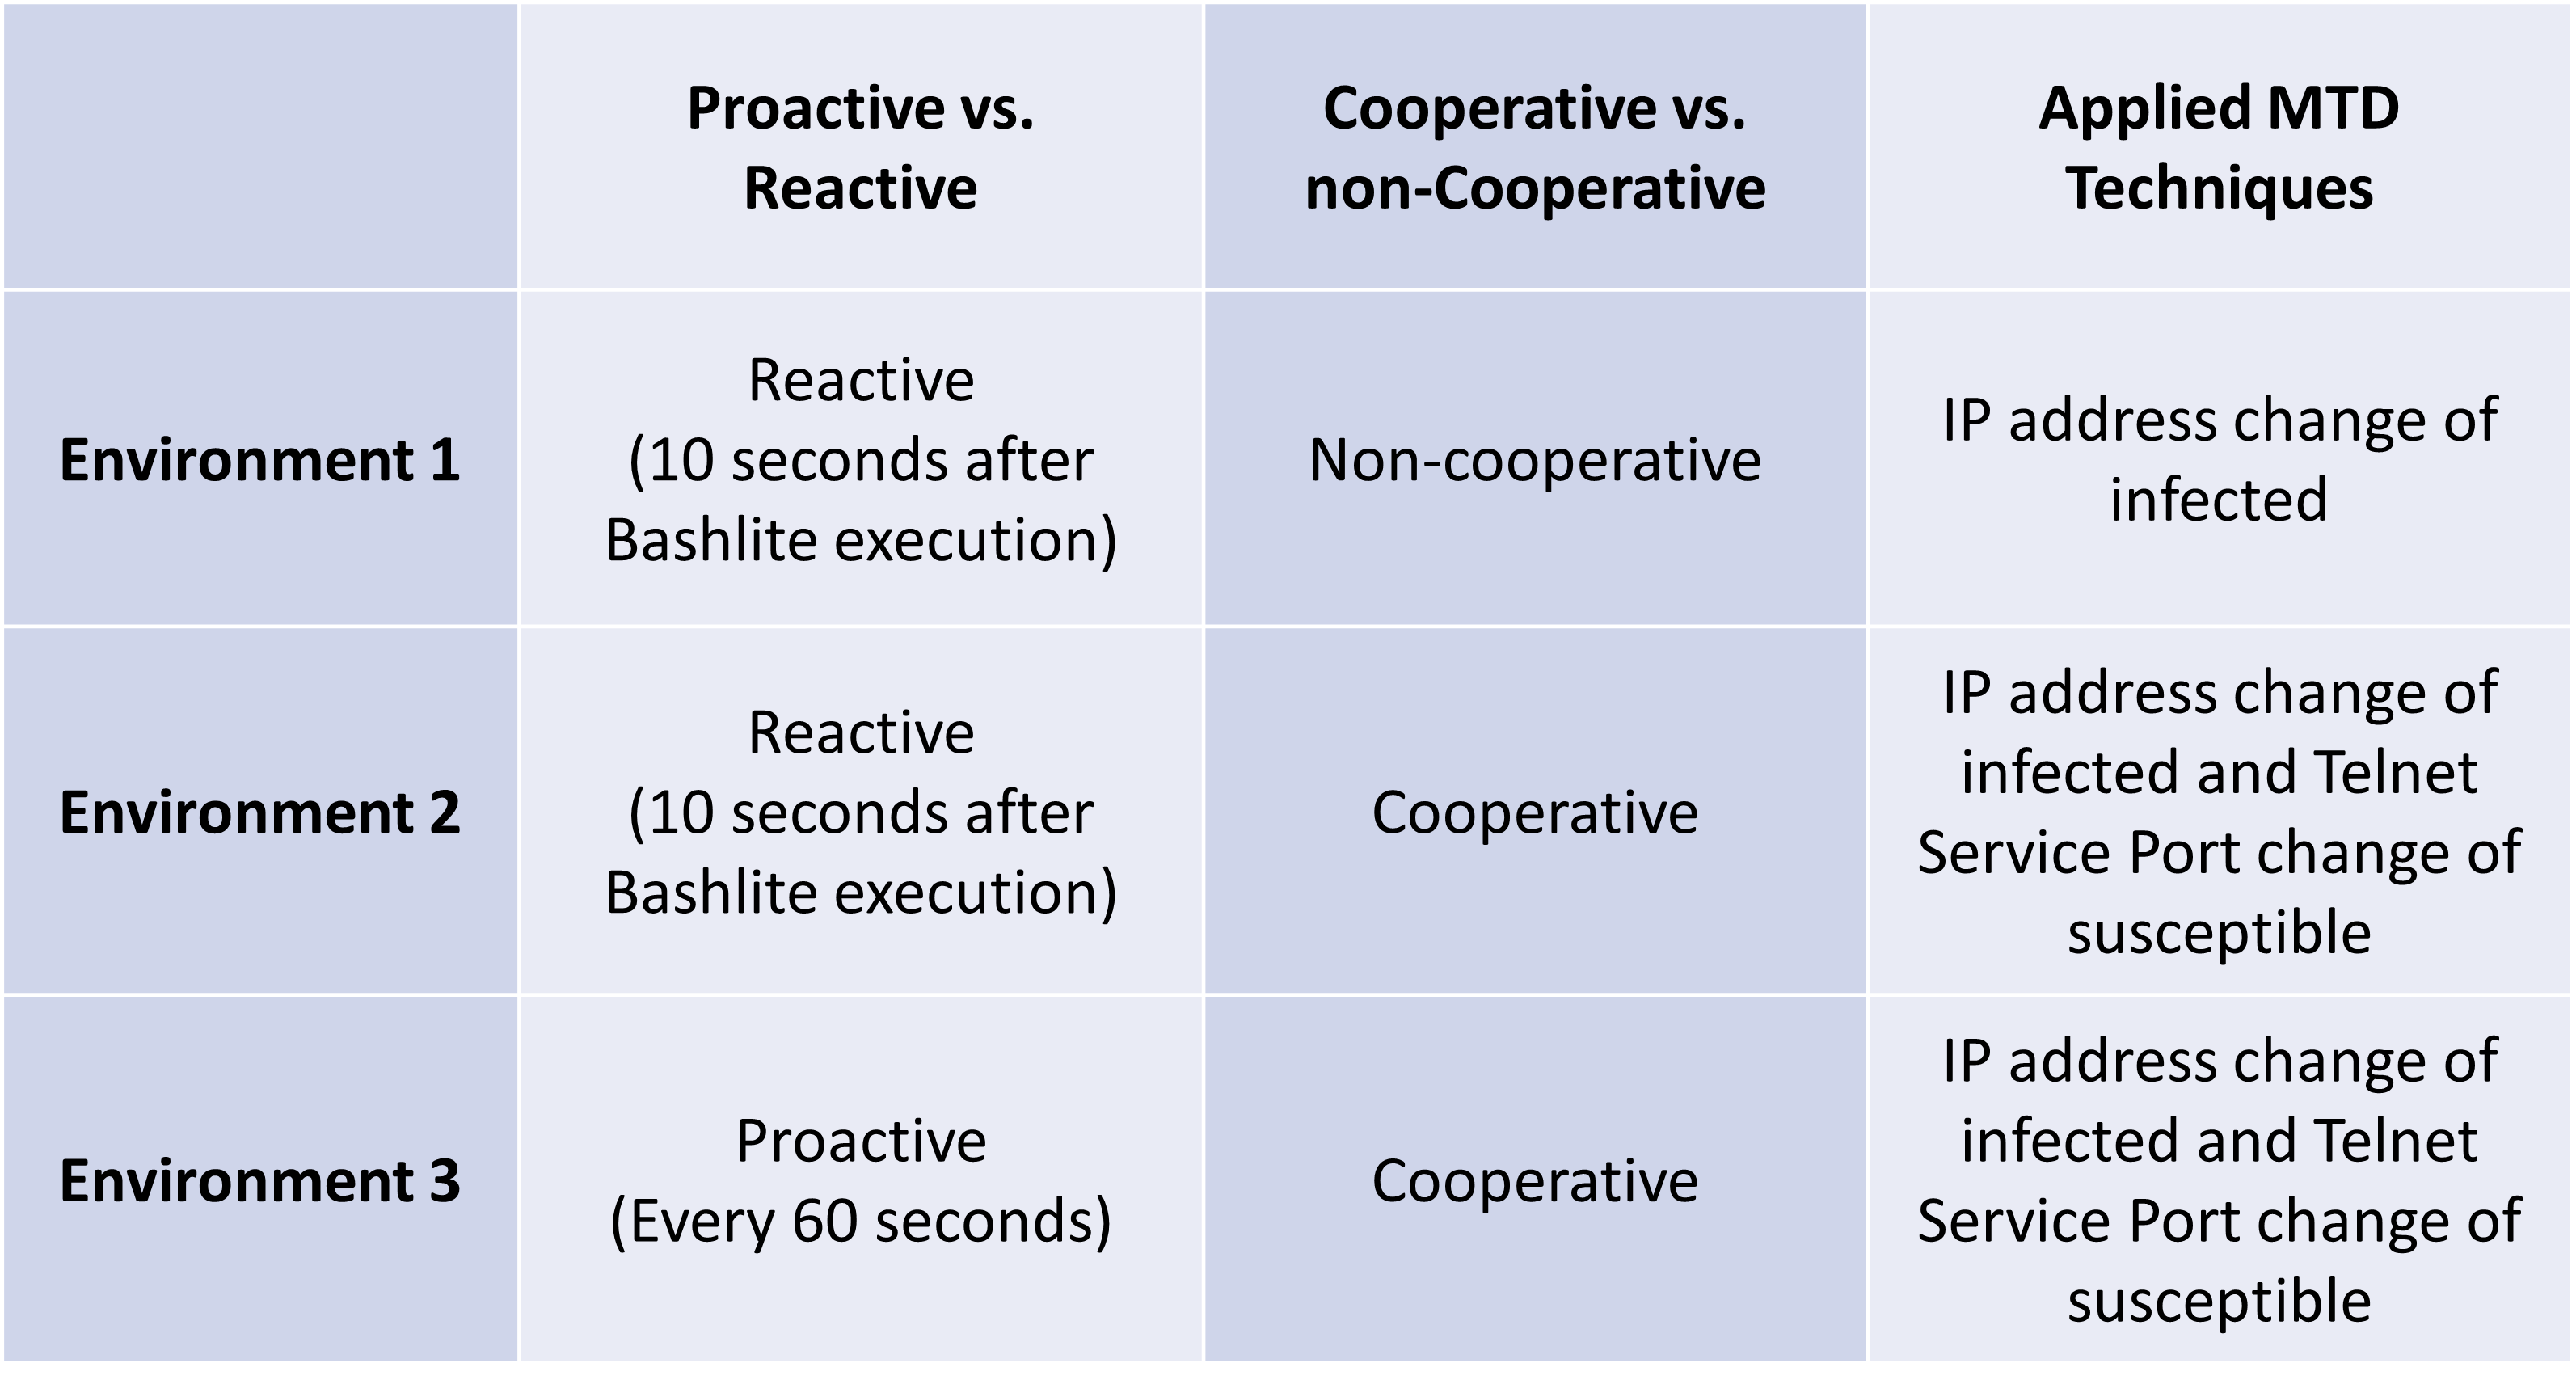
\includegraphics[scale=0.65]{assets/tableEvaluationEnvironment.png}
\centering
\caption{A Table Showing the Characteristics of Three Different Environments in Which the Previously Defined Metrics are Measured.}
    \label{graphic:tableEvaluationEnvironment}
\end{table}




\section{Prerequisites for the Evaluation}
Even though the implemented MTD mechanism worked, its code had to be adapted on several occasions. This involved three main tasks:
\begin{enumerate}
\item Writing scripts to measure and log the metrics, such as how long Bashlite has been running on the machine. 
\item Automating the code as much as possible. To get a reasonable amount of data, the infection/mitigation process had to be run multiple times, which was not feasible by hand. The idea was to be able to run the whole process once and then repeat it \textit{n} times.
\item Modifying the current scripts to fit the different environments. This included, for example, the adaptation that no Telnet service port change was triggered in Environment 1.
\end{enumerate}

The following subsections briefly describe how these tasks were accomplished. However, first an important aside regarding the Bashlite client. There was the problem that it was not possible to check whether a Bashlite client was still connected to the Bashlite server or not. To solve this, the killing of the Bashlite client in the IP address change technique remained in the code. This was justified by extensive testing and the existing literature~\cite{article:vonderAssen} regarding the interruption of the connection between the server and the client, and because the evaluation would simply not have been possible otherwise. Moreover, Bashlite is killed as soon as the client loses connection to the server, so there is only a negligible difference in time. This allowed the simplification that if a Bashlite client was running on the system, it was also connected to the server and vice versa. 


\subsection{Data Collection} \label{section:gatheringData}
Having solved this problem, a mixture of Bash and Python scripts were written to log the data into some .csv files, which were later analysed and plotted using Python. The reason for using both types of script was that sometimes one or the other was more suitable. This resulted in several files. 

The \textit{stopTimeOfClient.sh} script checks every 0.05 seconds whether the client process is running on the machine. If it is, the script stores the time of the start of the client, waits for it to finish and writes all the information to a \textit{bashliteAnalysis.csv} file. This script is continuous and also indicates which Bashlite run the system is on.

The \textit{CPURamAnalysis.py} script uses \textit{psutil} to monitor the CPU and RAM usage of the system and writes this to a CPURamAnalysis.csv file. The original idea was to specifically measure the CPU and RAM usage of the script that executes the MTD techniques on each machine. However, as the CPU usage of the script was almost always 0\% (measured with Bash/top and Python/psutil to exclude errors), a graph showing this would not give much insight. Thus, only the RAM usage was measured with \textit{psutil} since this was giving correct and measurable results. The CPU usage of the infected and susceptible machines was measured once with the MTD mechanism deployed and techniques executing, and once without the MTD mechanism deployed. This allowed to compare the case with MTD to the case without MTD on the respective machine. Both measurements were run for 15 infection/mitigation runs, equivalent to 30 minutes.  

%This gives a indication about how hardware intensive the actual execution of the MTD techniques is, since for example the IP change is only executed when Bashlite is active. Thus, it was possible to compare the system without executing MTD techniques against the system where the MTD are executed and Bashlite is active. The maximum CPU used can therefore not be higher than the difference between these two cases. Another reason why this approach made sense is that the defense mechanism on the clients are intended to run permanently, because they need to listen to potential attacks. 

The \textit{sendPacketsToServer.sh} script monitors outgoing packet losses. This is achieved by sending simple one-packet pings to the server machine every 0.5 seconds. The script also keeps track of the current Bashlite run. This gives interesting insights for the different environments. In Environment 1 and 2, outgoing packet losses should only occur once per Bashlite run, as the MTD techniques are executed reactively. In Environment 3, the MTD techniques are executed proactively, and therefore multiple packet losses are possible during a Bashlite run. All this information is written to a \textit{packetLoss.csv} file.

The \textit{telnetToLocal.py} and \textit{telnetToLocalOnlyIP.sh} scripts were written to track the interruption of the incoming Telnet service from the susceptible machine. The former was created first and uses \textit{sockets} (or \textit{telnetlib}) to check whether port 23 of the executing machine is listening or not. This produced reliable results, but there was an issue in the non-cooperative environment due to the two possible IP addresses the susceptible machine could have. Sockets in general were too slow to either get the host IP address or try to connect to both possible IP addresses, so a shell script that uses \textit{netcat} to check whether port 23 of both possible IP addresses are listening was more suitable. All this information is logged to a file called \textit{telnetToLocal.csv} or \textit{telnetToLocalOnlyIP.csv} depending on which script was used.

The \textit{telnetToServer.py} file is the last script and monitors whether outgoing telnet connections are possible or not. It does this using the \textit{telnetlib} module as in this case, it was essential to use Telnet as the communication protocol for the outgoing connection. 

%\todo{es wär mega guet zum eh grafik mache woni d'vms han, iwie usgehendi und ihkommendi pfiil wo ahgebed wele weles file was catcht }



\subsection{Automation}
Regarding automation, the implementation code already fulfilled most of the requirements. Only four issues remained. The first was that the script \textit{sendToDeployerClient.py} from VM1 needed some adaptations to separate the start of Bashlite from the start of the defence technique (notifying the \textit{Deployer Client}). One reason for this was the parent/child relationship between Bashlite and the Python script, which made it impossible to kill Bashlite (the child) while the Python script (the parent) was still running. Creating another Bash script called \textit{startBashAndSendToDepClient.sh} solved this problem. This file contains a while loop with each iteration being an entire infection/mitigation process. First, the while loop starts the Bashlite client and then sleeps for 10 seconds, mimicking the time it takes to detect Bashlite. After this time it starts the \textit{sendToDeployerClient.py} in the background and then sleeps again for 110 seconds. This time period could also be shorter, but it ensured that the previous infection process is completed with all the corresponding MTD techniques. 

The second problem was that the \textit{sendToDeployerClient.py} script had to be triggered somehow on VM2 as well. It was not possible to use the same script as for VM1 (\textit{startBashAndSendToDepClient.sh}), since this started Bashlite manually on VM1 and VM2 needed to detect it somehow. The solution was a Bash script that runs continuously and checks if Bashlite is running. If Bashlite is running for more than 10 seconds, the script executes \textit{sendToDeployerClient.py} which then initialises the MTD mechanism. This functionality was implemented with a shell script called \textit{checkForBashliteAndStartMTD.sh}. 

The third encountered issue was that the Bashlite server would only allow one infection, after which a restart of the server was required. This was added at the beginning of the thesis to improve stability, as the Bashlite client was constantly sending the same report about the susceptible machine, causing the Bashlite server to crash. Since it was not an option to always restart the server manually, the Bashlite client was adapted to send the report only once, and thus the restriction on the Bashlite server could be removed. 

The fourth issue was that about 15 scripts per environment would have had to be started to get everything running. To avoid this, a Bash script (\textit{runAll.sh}) was written containing all the startup instructions for each machine and environment. This resulted in three different startup scripts on three different machines, which was acceptable. Additionally, the counterparts for terminating all scripts started by \textit{runAll.sh} were created. This allowed to quickly start all the scripts, let them collect data and then terminate them effortlessly.

\subsection{Creating Evaluation Environments}
Finally, the different environments/systems had to be created. The first environment was the non-cooperative one, which only involved changing the IP addresses of the infected machines. 
The only required server-side adaptation was to instruct the \textit{Deployer Server} not to initiate any Telnet service port changes. This was done by replacing the array containing all the IP addresses that were potentially going to receive a port change with an empty array. 

On the client side, there was the problem that the Bashlite client was only scanning one IP address for a susceptible machine, so as soon as the IP address change was executed on VM2, the Bashlite client on VM1 would no longer find VM2 in the next Bashlite run. To solve this, two hardcoded IP addresses replaced the IP address variable received from the \textit{Deployer Server}. Thus, VM2 simply switches between these two IP addresses instead of migrating to the one sent by the \textit{Deployer Server}. This allowed adapting the Bashlite scanner of the client of VM1 to try only two different IP addresses, which worked perfectly. Note that this was only needed for the evaluation as the Bashlite implementation is limited. If it were not for the evaluation, or if Bashlite was scanning in a more sophisticated way, this adaptation would not be required at all. Besides, this did not make any difference to the data collected.

The second environment was the original idea, which was Bashlite together with a cooperative MTD approach. Since this usecase was the goal from the start, nothing had to be changed. The third environment involved Bashlite with the proactive MTD execution. To create this environment, the only required adaptation was to split the \textit{startBashAndSendToDepClient.sh} script into two subscripts. The first script starts the MTD mechanism every 60 seconds, the second script starts Bashlite randomly at an interval between 60 and 90 seconds. These two scripts are then executed by the \textit{runAll.sh} script. 




\section{Results} \label{section:results}
This section presents the results of the evaluation. It is divided into the three metrics mentioned in Section \ref{section:evaluationMethodology}, namely the duration of infection activity in the network, the interruption of availability, and the CPU/RAM usage. 

\subsection{Duration of Infection Activity in the Network}
The duration of infection activity was the most important metric as it defined whether the defence mechanism was working or not. Figure \ref{graphic:tableEvaluationEnvironment} shows the results for Environment 1, which was the non-cooperative and reactive solution. On the x-axis is the current run (infection/mitigation process). The blue bar of the stacked bars shows the number of seconds that VM1 was infected with Bashlite, meaning that Bashlite lasted approximately 29 seconds on VM1 in each run. The orange bar shows the number of seconds that VM2 was infected, which was also approximately 29 seconds per run. This gave an average of 57.6 seconds of total infection activity on the two VMs per run. It is evident that in this non-cooperative approach, the spreading to the susceptible machine could not be prevented at all. Bashlite was still mitigated, but each machine had to clean itself after the infection had occurred. 

\begin{figure}[tph]
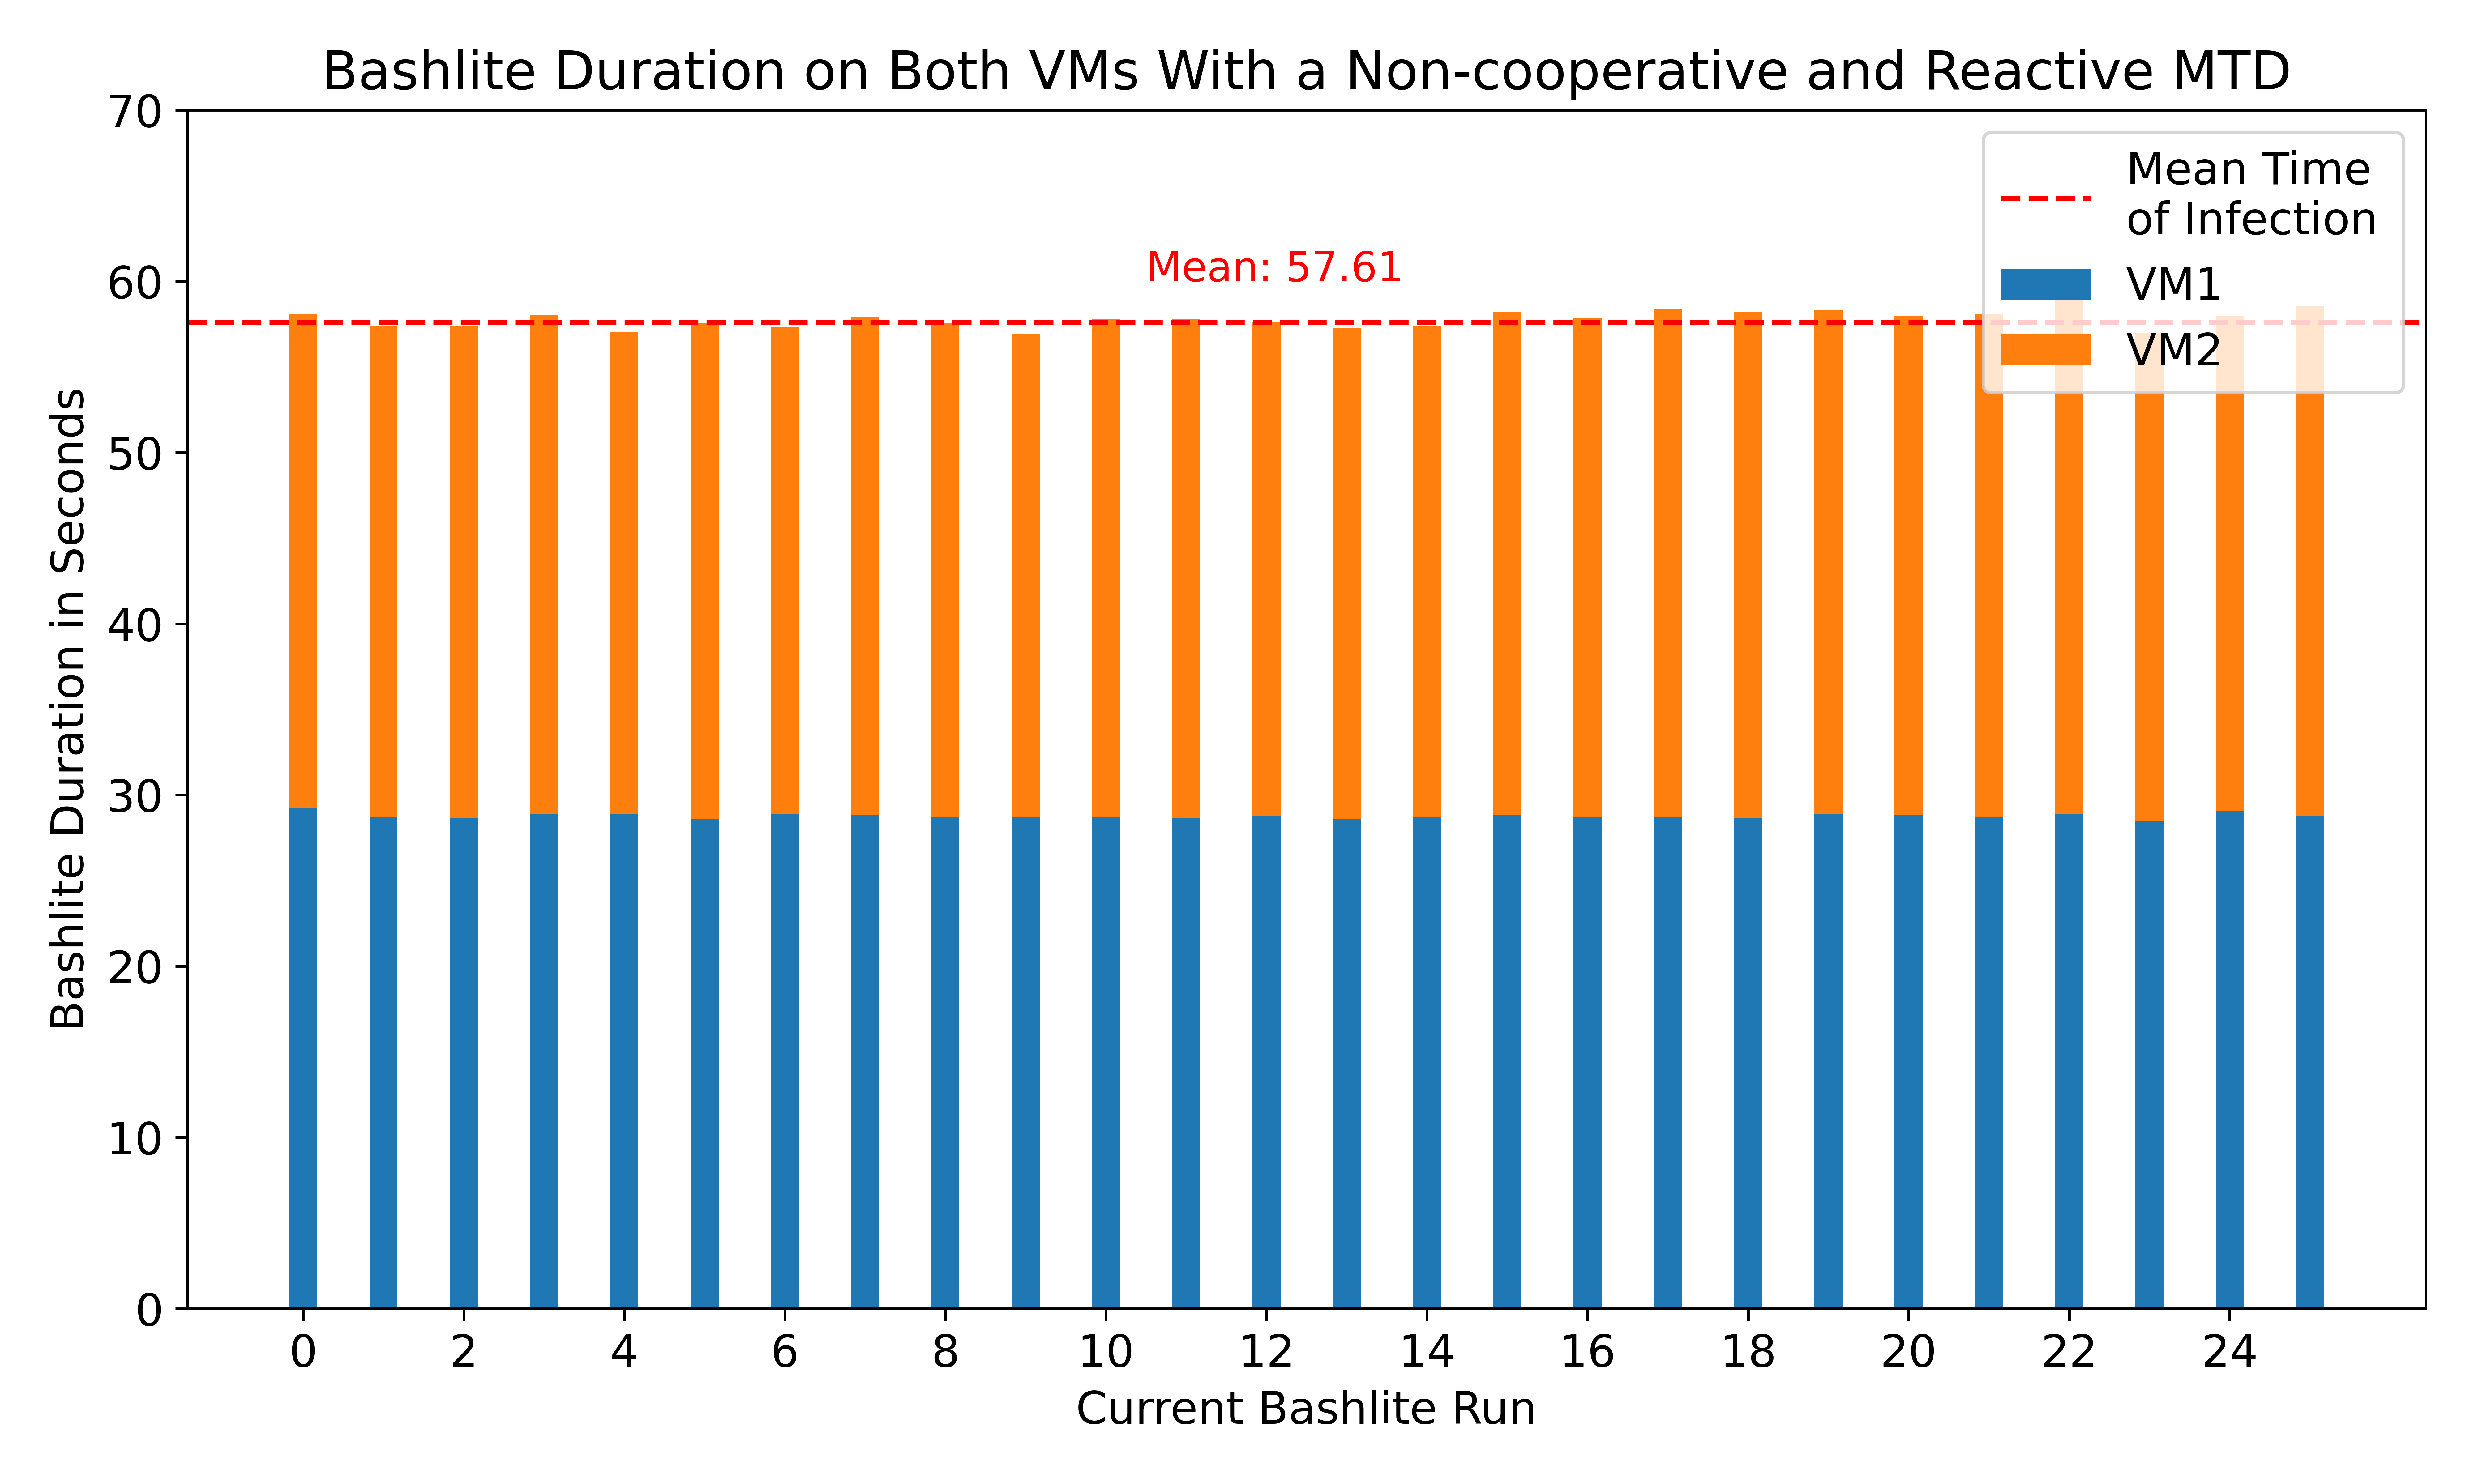
\includegraphics[scale=0.6]{assets/bashliteDurationUncoopAndReactive.png}
\centering
\caption{The Duration of Infection Activity on Both Virtual Machines in the Non-cooperative and Reactive Environment.}
\label{graphic:tableEvaluationEnvironment}
\end{figure}

Figure \ref{graphic:bashliteDurationCoopAndReactive} shows Environment 2, which was the cooperative and reactive environment. Again, the blue bars represent the number of seconds that VM1 was infected, the orange bars would represent the time that VM2 would have been infected if this had occurred. It is evident that in the cooperative and reactive environment the spreading to VM2 was prevented in every run. This resulted in an average of about 28.8 seconds of total infection activity on the two VMs, which is approximately half of the time of the uncooperative and reactive environment. 






\begin{figure}[tph]
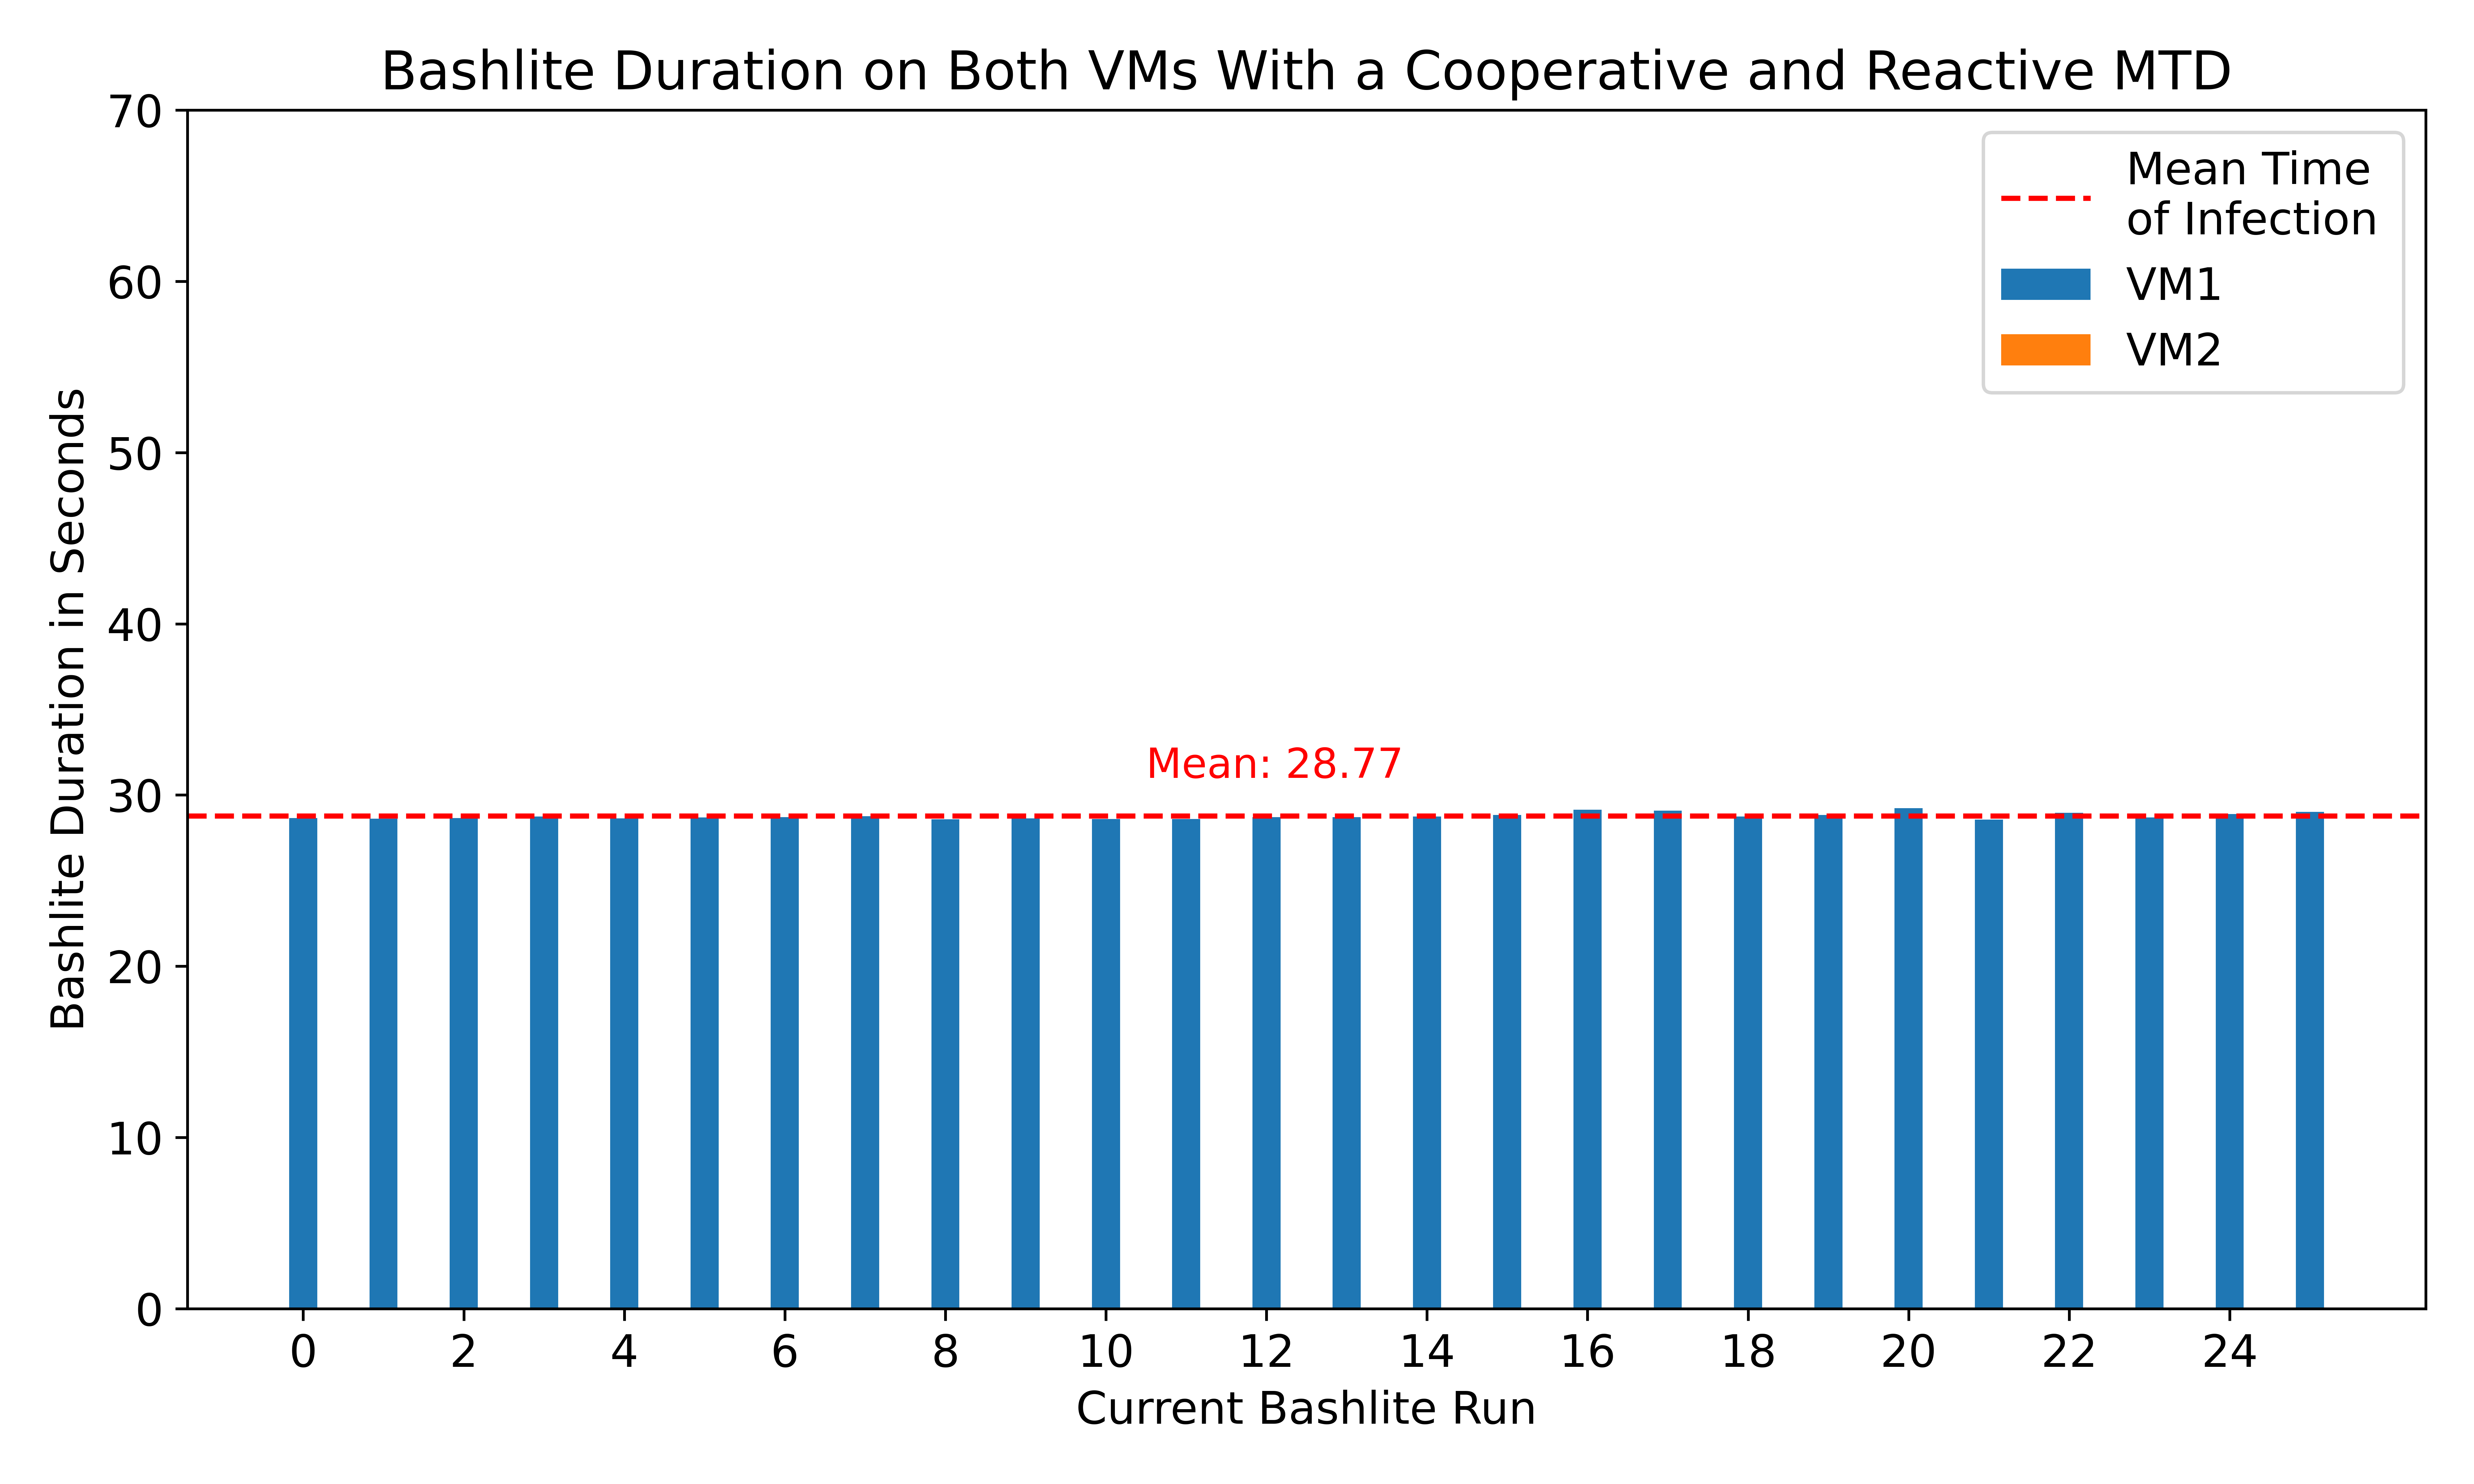
\includegraphics[scale=0.6]{assets/bashliteDurationCoopAndReactive.png}
\centering
\caption{The Duration of Infection Activity on Both Virtual Machines in the Cooperative and Reactive Environment.}
\label{graphic:bashliteDurationCoopAndReactive}
\end{figure}


Figure \ref{graphic:bashliteDurationCoopAndProactive} shows Environment 3, which was the cooperative but proactive environment. Unlike the previous two environments, the Bashlite duration was different for each run. The mean duration was slightly higher than the mean duration of the cooperative and reactive environment, but much lower than that of the non-cooperative and reactive environment.   





\begin{figure}[tph]
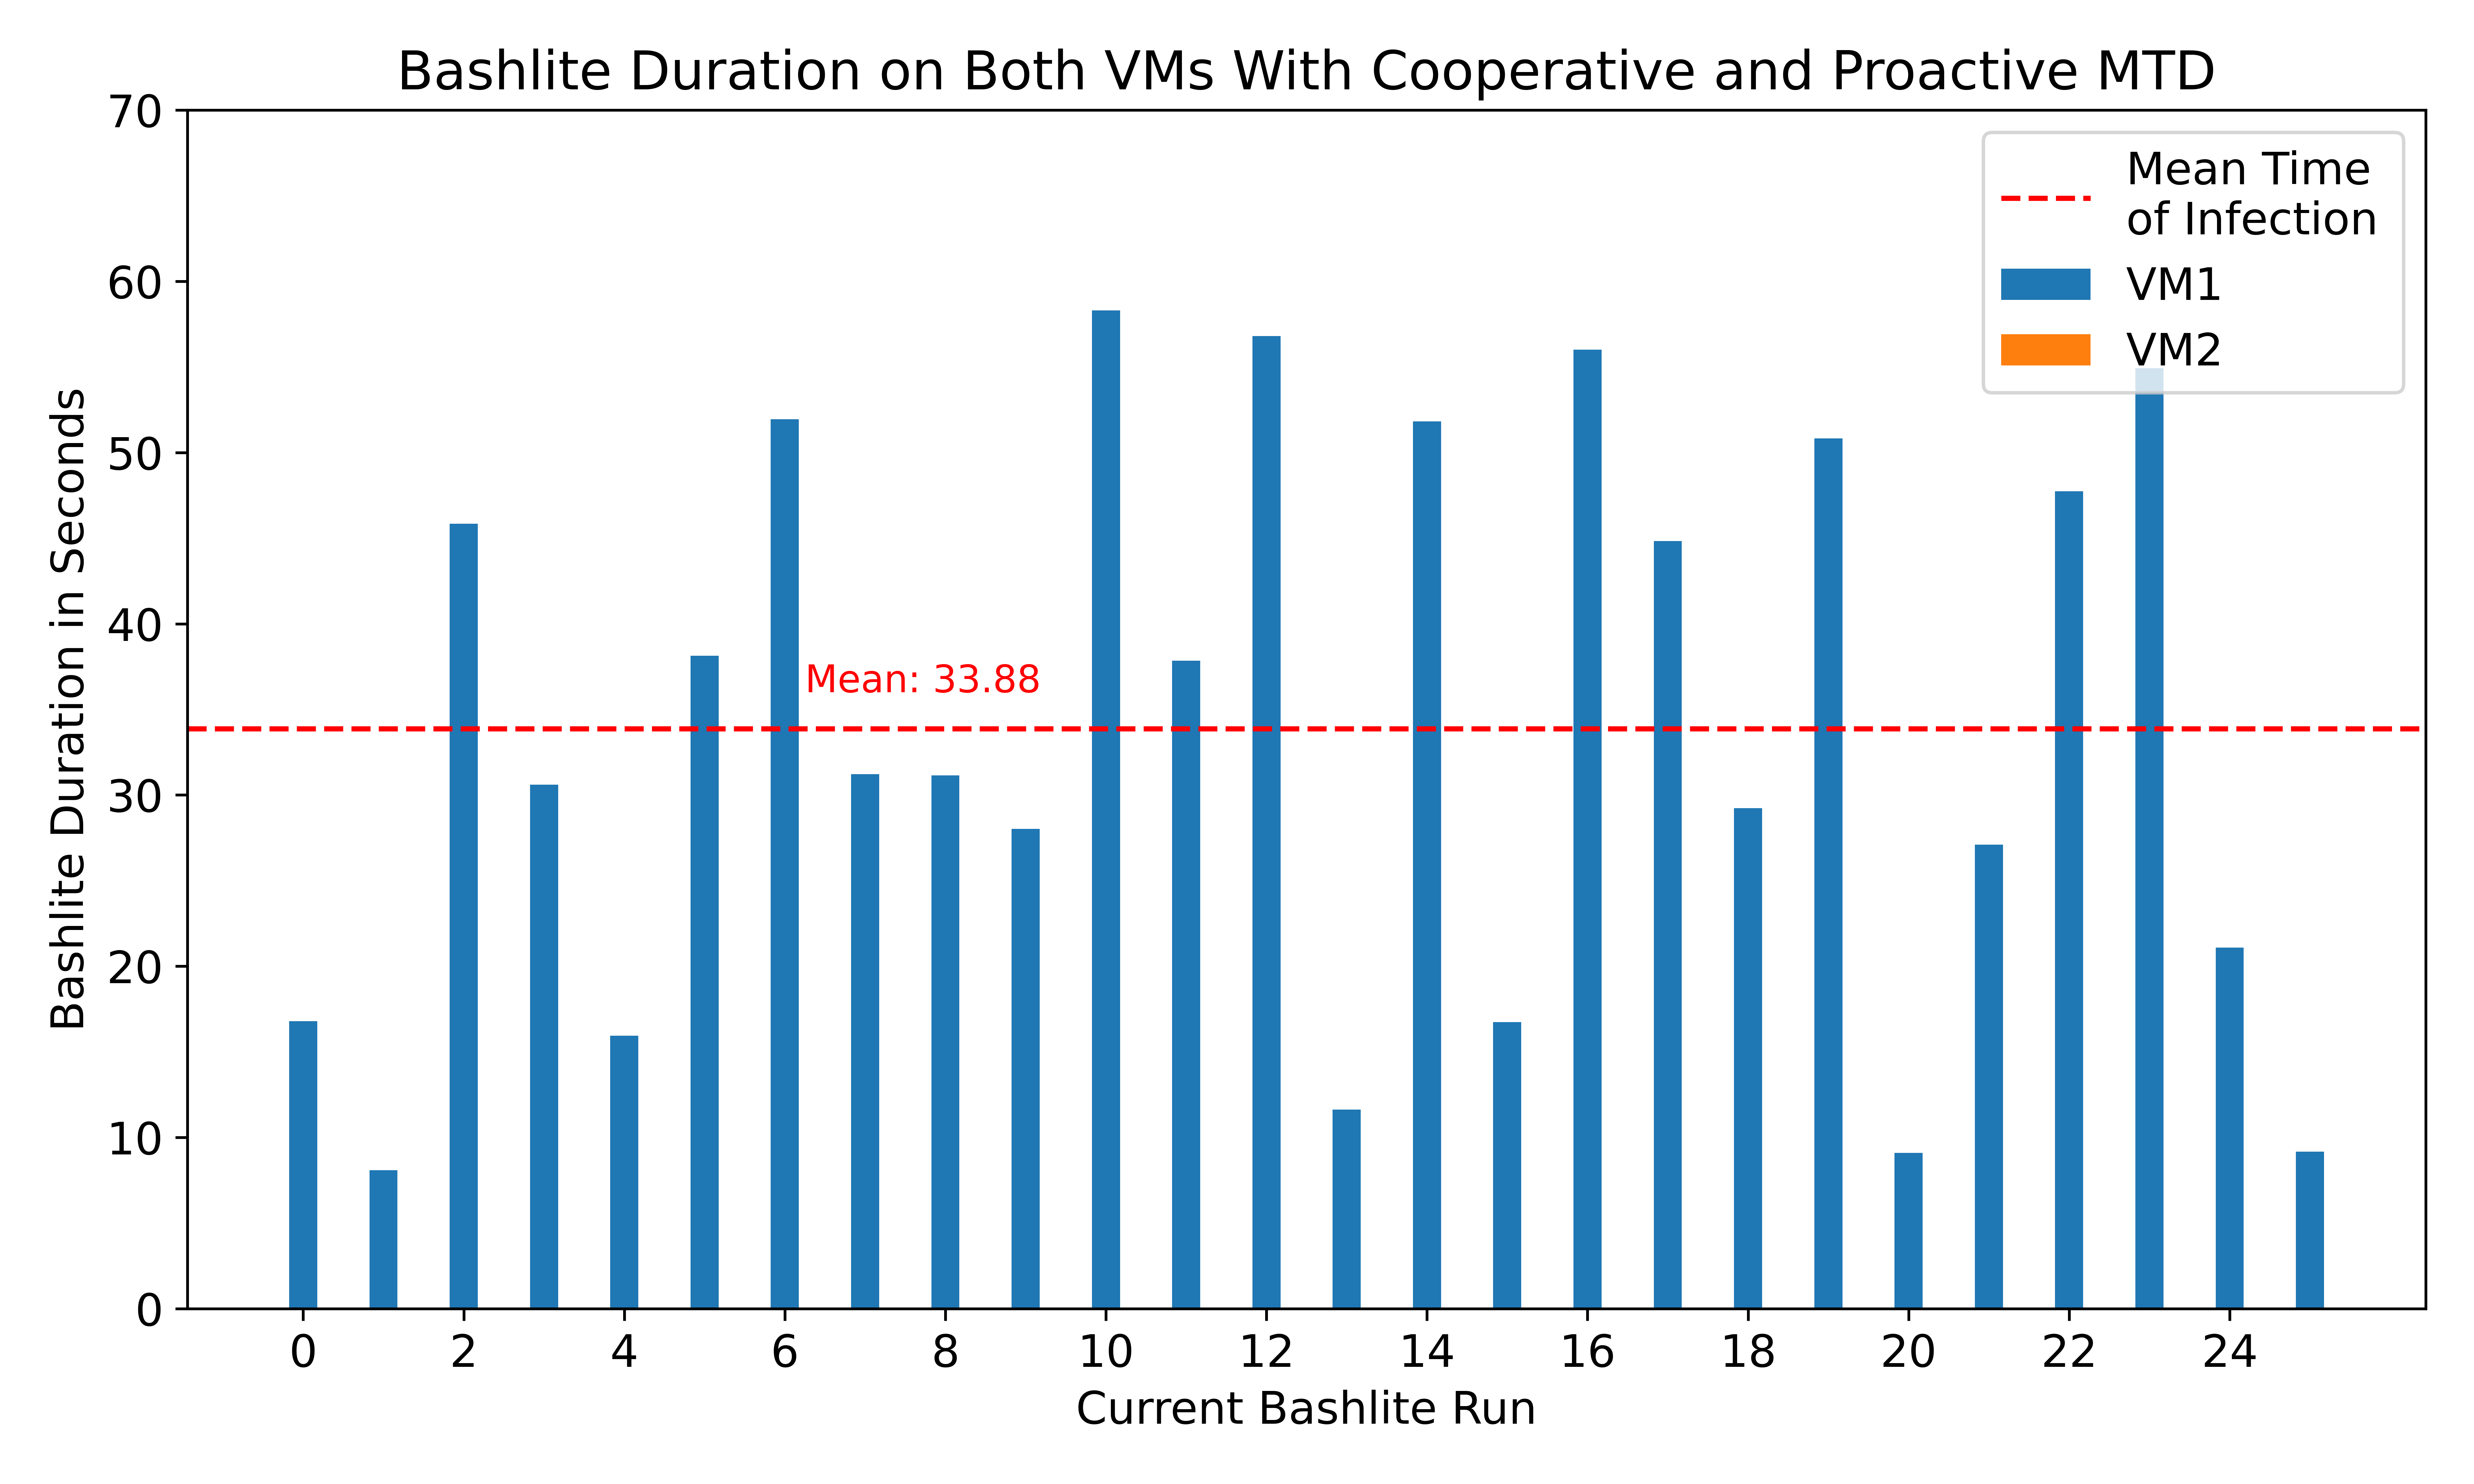
\includegraphics[scale=0.6]{assets/bashliteDurationCoopAndProactive.png}
\centering
\caption{The Duration of Infection Activity on Both Virtual Machines in the Cooperative and Proactive Environment.}
\label{graphic:bashliteDurationCoopAndProactive}
\end{figure}


Figure \ref{graphic:bashliteDurationSummary} shows the duration of the average total infection activity on VM1 and VM2 over 25 runs. The cooperative and reactive environment had the shortest duration of infection activity, the cooperative and proactive environment followed immediately and the non-cooperative and reactive environment had by far the longest average duration of infection activity. This was due to the infection of the susceptible machine.

\begin{figure}[tph]
\includegraphics[scale=0.4]{assets/bashliteDurationSummary.png}
\centering
\caption{A Summary of all Three Environments and Their Respective Infection Duration.}
\label{graphic:bashliteDurationSummary}
\end{figure}


\subsection{Interruption of Availability}
Figure \ref{graphic:packetLossSummary} shows the share of packet losses out of the total packets sent by the two VMs in all three environments. Environment 1, which executed the IP address change on both machines on every run due to the uncooperative nature, had the highest packet loss with about 4.2\%, the remaining 95.8\% were successfully delivered. Environment 2, which consisted of the cooperative and reactive MTD, had by far the lowest packet loss with about 2.1\%. Environment 3 with the cooperative and proactive approach had a similar packet loss as Environment 1. 

\begin{figure}[tph]
\includegraphics[scale=0.4]{assets/packetLossSummary.png}
\centering
\caption{A Summary of all Three Environments and Their Respective Average Share of Outgoing Packet Losses From all Packets Sent.}
\label{graphic:packetLossSummary}
\end{figure}

The incoming Telnet connection showed a different picture than the packet losses, as shown in Figure \ref{graphic:telnetToLocalSummary}. Environment 1 had by far the lowest share (4.2\%) of failed incoming Telnet connections of all incoming Telnet connections. This was due to the fact that no Telnet port changes were involved here (only the IP address change). Environment 2 was in the middle with a share of 31.6\% failed incoming Telnet connections and Environment 3 had by far the highest share of failed Telnet connections with 61.4\%. 

In addition to the incoming Telnet connections, the outgoing Telnet interruptions were also measured. It was evident that changing the Telnet port did not interrupt or prevent any outgoing connections. The only time that outgoing Telnet connections were not possible was when the IP address of the device changed. Therefore, the interruption of outgoing Telnet connections was the same as the share of outgoing packet losses shown in Figure \ref{graphic:packetLossSummary} for every environment. This means that in the non-cooperative and reactive environment
and the cooperative but proactive environment, approximately 4.2\% of outgoing Telnet connections failed. In the cooperative and reactive environment, around 2.1\% of outgoing Telnet connection failed.



\begin{figure}[tph]
\includegraphics[scale=0.4]{assets/telnetToLocalSummary.png}
\centering
\caption{A Summary of all Three Environments and Their Respective Average Share of Failed Incoming Telnet Connections.}
\label{graphic:telnetToLocalSummary}
\end{figure}



\subsection{CPU and RAM Usage}

Figure \ref{graphic:RAMUSageBoth} shows the constant RAM usage of the MTD mechanism over 30 minutes with the MTD techniques executed multiple times on both VMs. VM2 used a minimal amount more RAM, but this difference is negligible as it is in the byte range and the machines have gigabytes of available RAM. So in general, the mechanism's RAM usage was minimal.  

\begin{figure}[tph]
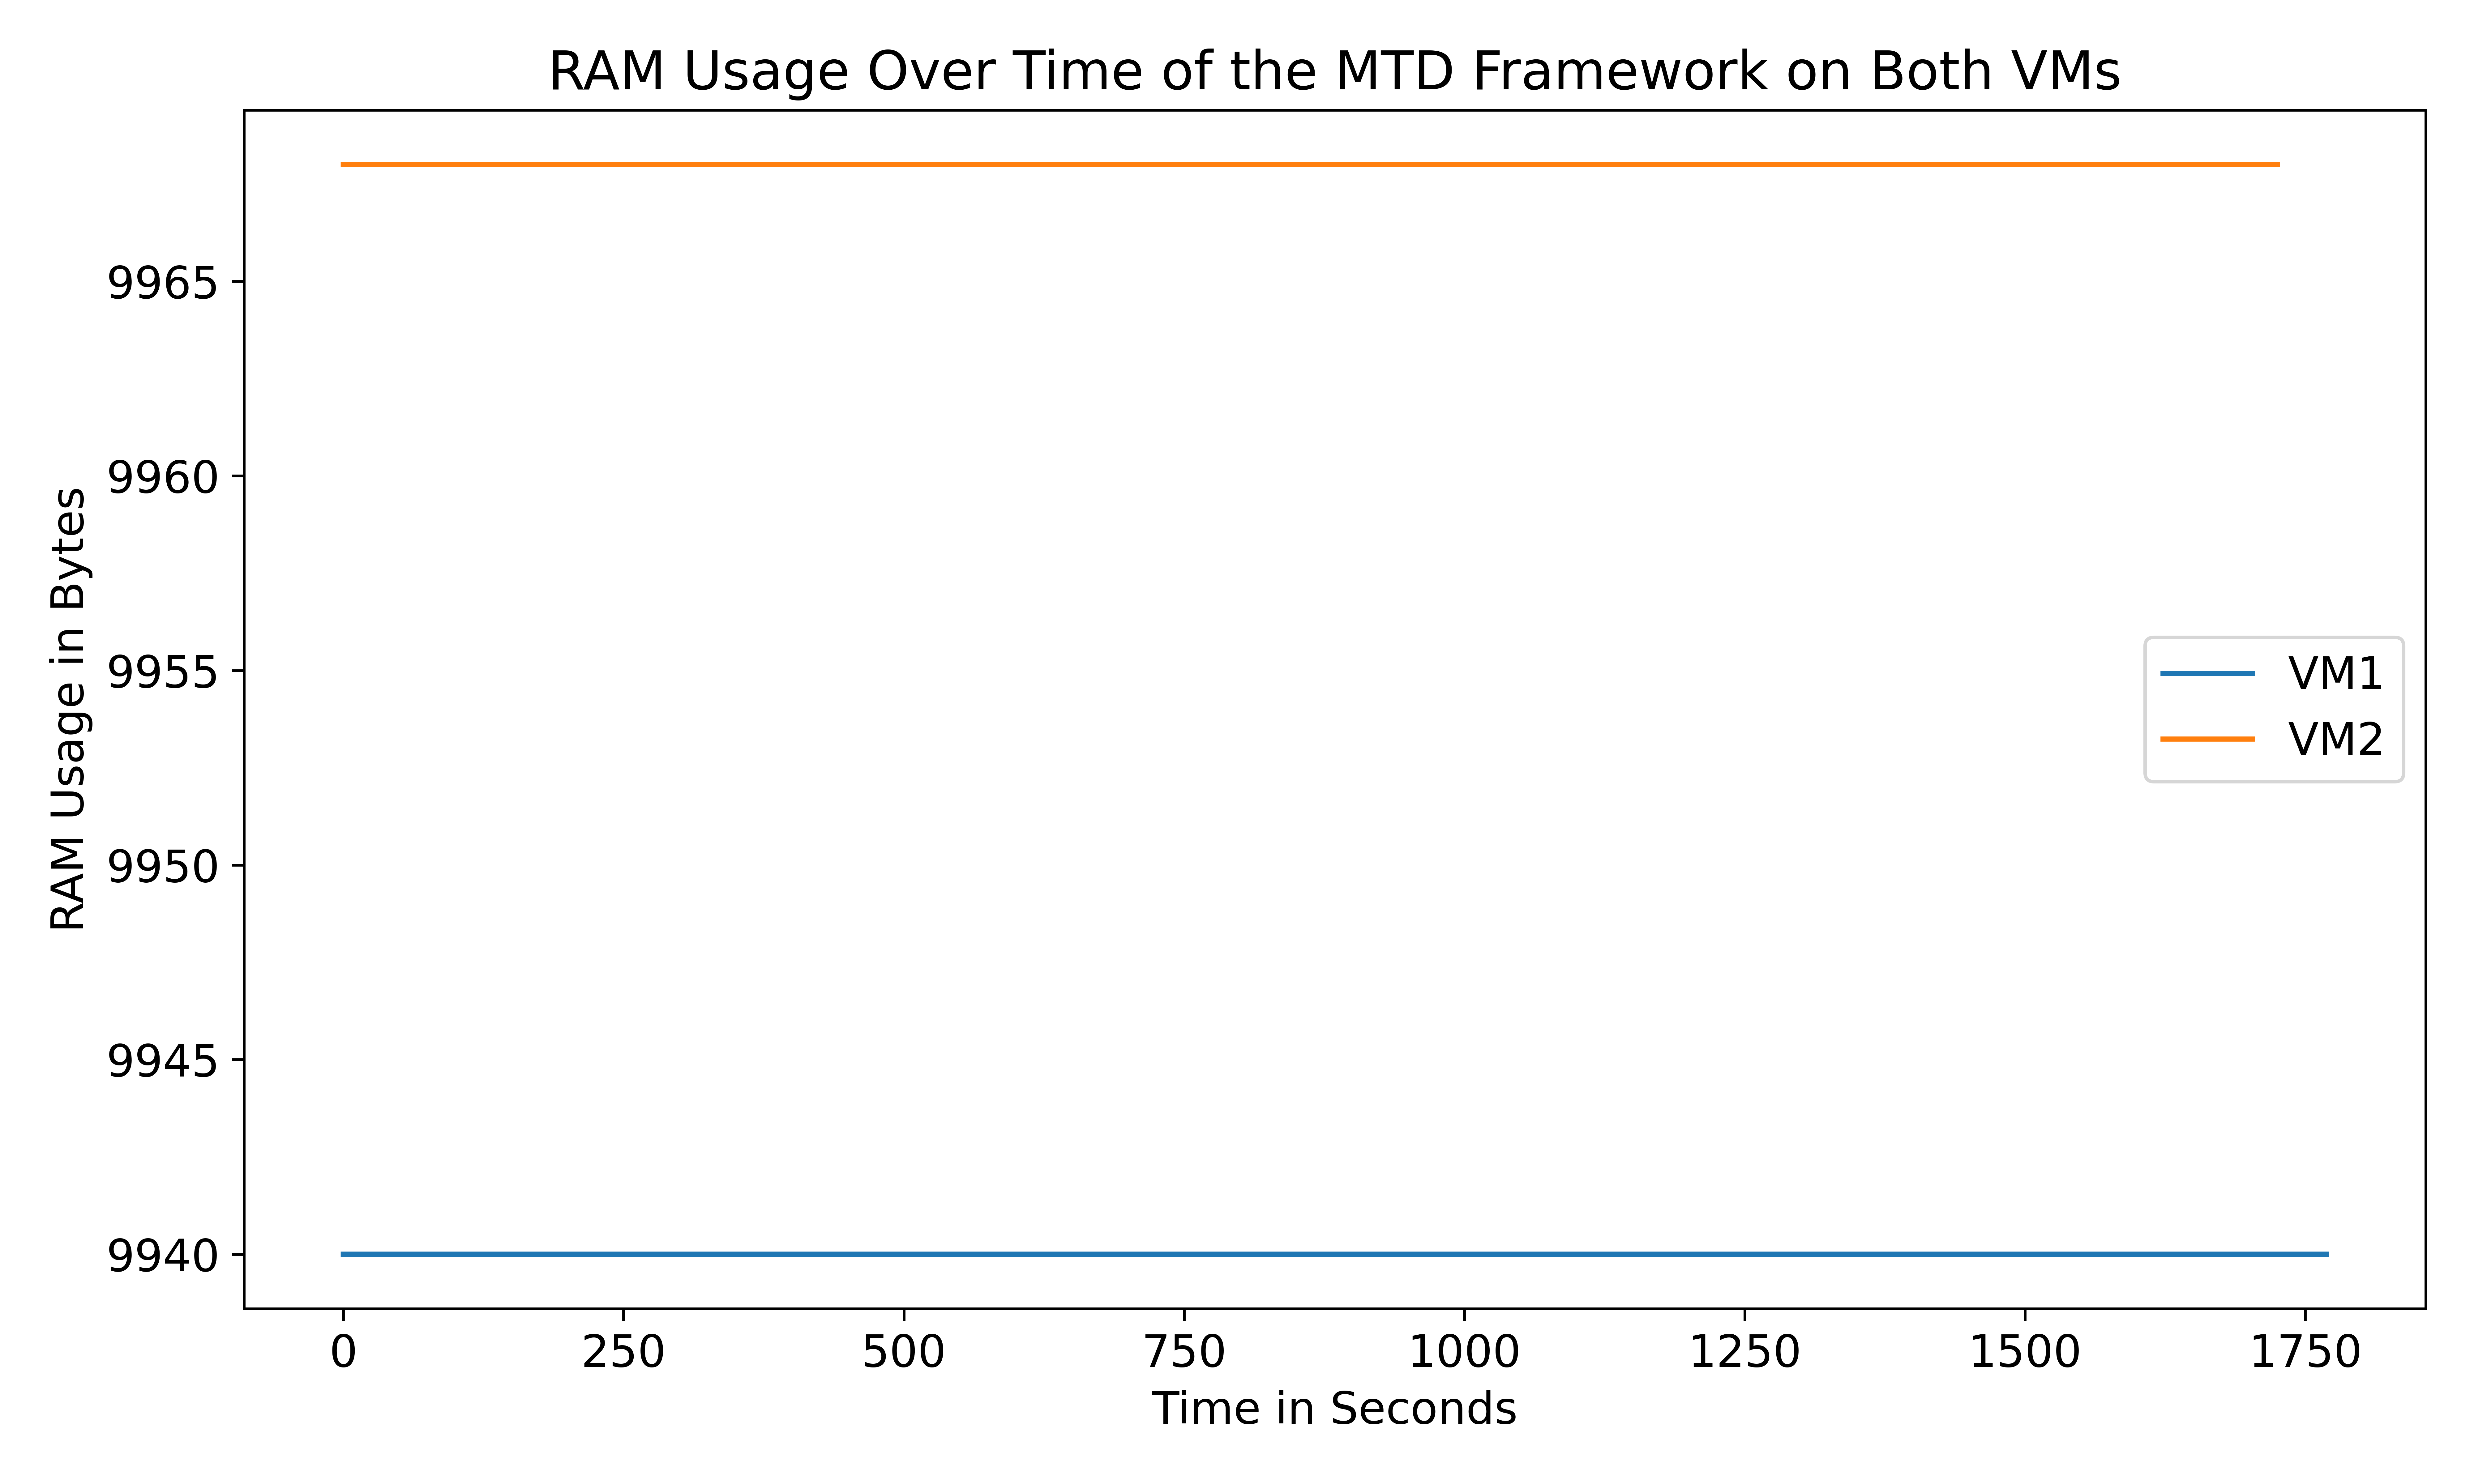
\includegraphics[scale=0.65]{assets/RAMUSageBoth.png}
\centering
\caption{The RAM Usage of the Running MTD Framework with Multiple Executions of the MTD Techniques on Both VMs.}
\label{graphic:RAMUSageBoth}
\end{figure}


Figure \ref{graphic:CPUVM1MTDNotDeployed} shows the CPU usage of VM1 without the MTD deployed. The CPU usage varied between 20\% and 32\% with only a few outliers that are higher. In this case, no other program or script was started except the measurement script, so these outliers must be caused by the operating system or some other automatically started process. The average CPU usage was 23.53\%. Figure \ref{graphic:CPUVM1MTDDeployed} shows the same information, but this time with the MTD framework deployed and the MTD techniques executing multiple times. On VM1 the MTD technique performed was the IP address change. It is clear that the fluctuation was higher with the MTD framework deployed, ranging from 20\% to about 40\%. The high peaks were periodic, but also rather short. The average CPU usage was 0.02\% higher with the MTD mechanism deployed than without it. 

Figure \ref{graphic:CPUVM2MTDNotDeployed} and Figure \ref{graphic:CPUVM2MTDDeployed} give the same information, but for VM2, which performed the Telnet service port change. Again, there was a range of 20\% to 30\% with a few higher outliers in the base case. The average was 23.79\%, which was slightly higher than the average CPU usage of the base case of VM1. The CPU usage of VM2 with the MTD framework deployed and the techniques executing also showed more fluctuation than the base case of VM2. The average CPU usage of the deployed case was also slightly higher, namely 0.43\%. Although there were fewer high peaks on VM2 with the MTD mechanism deployed than in the respective case of VM1, the average CPU usage was higher on VM2 than on VM1.
\begin{figure}
     \centering
     \begin{subfigure}[b]{0.8\textwidth}
         \centering
         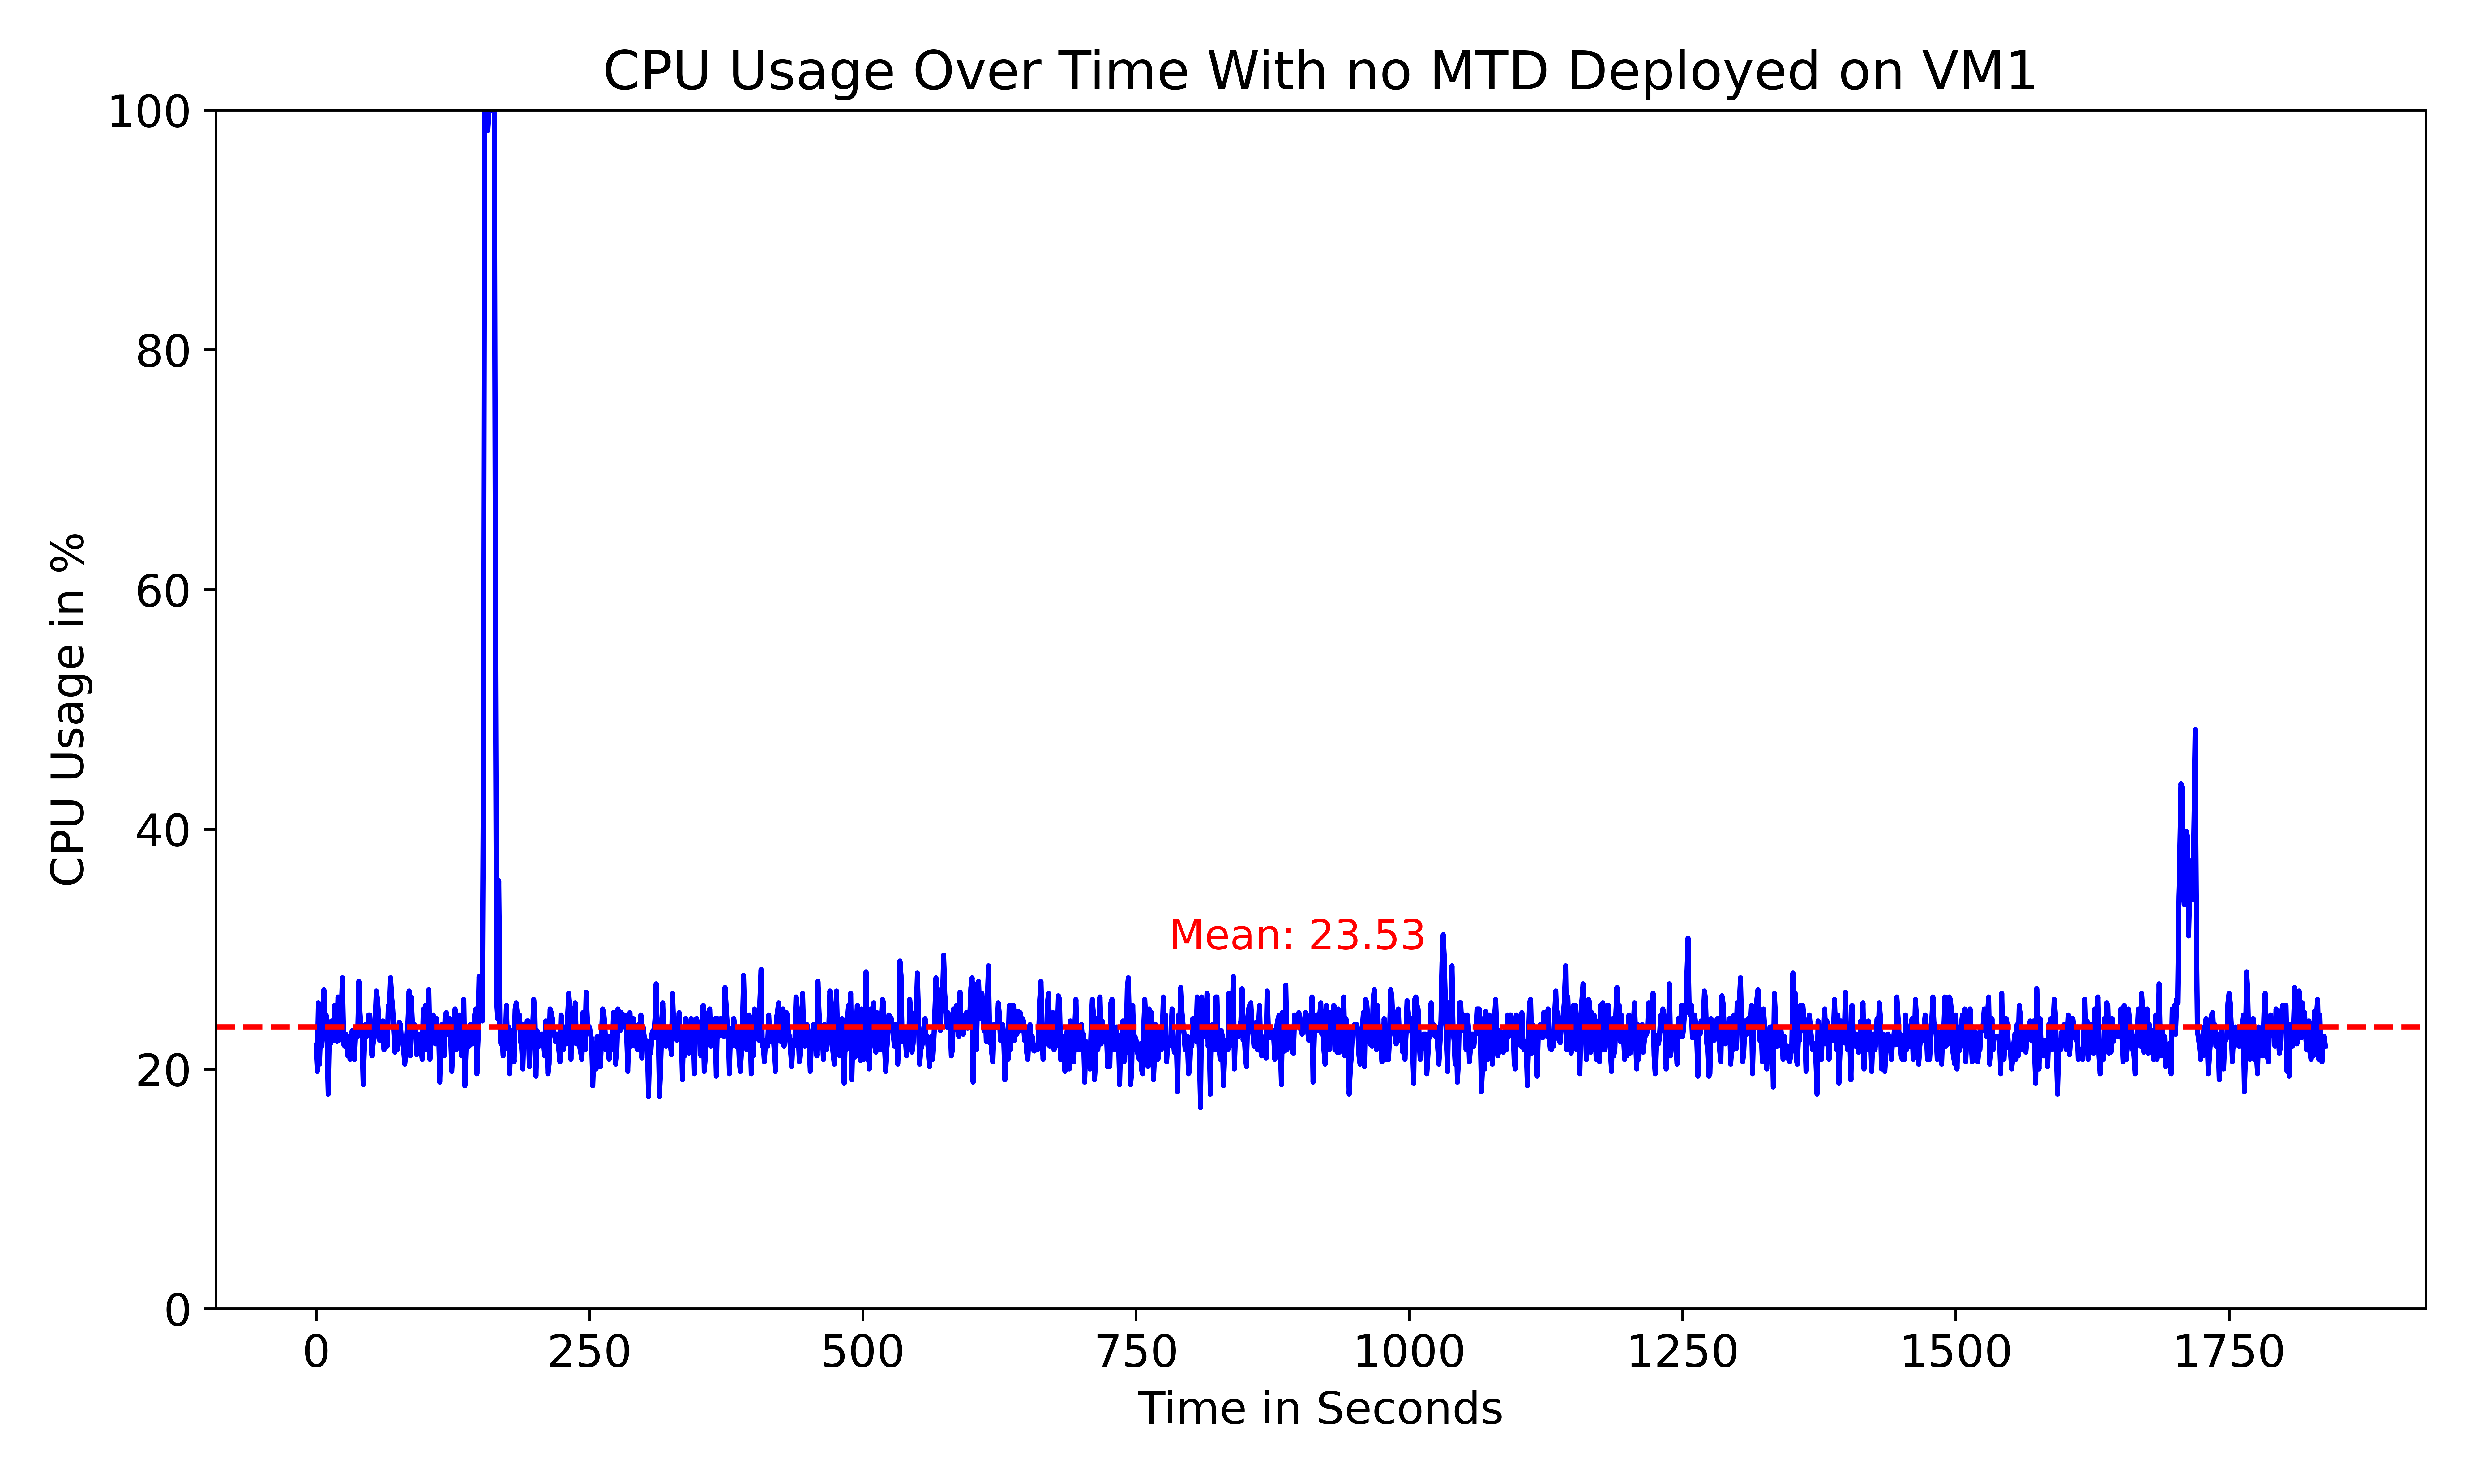
\includegraphics[width=\textwidth]{assets/CPUVM1MTDNotDeployed.png}
         \caption{The CPU Usage of VM1 Without the MTD Mechanism Deployed.}
         \label{graphic:CPUVM1MTDNotDeployed}
     \end{subfigure}
     \hfill
     \begin{subfigure}[b]{0.8\textwidth}
         \centering
         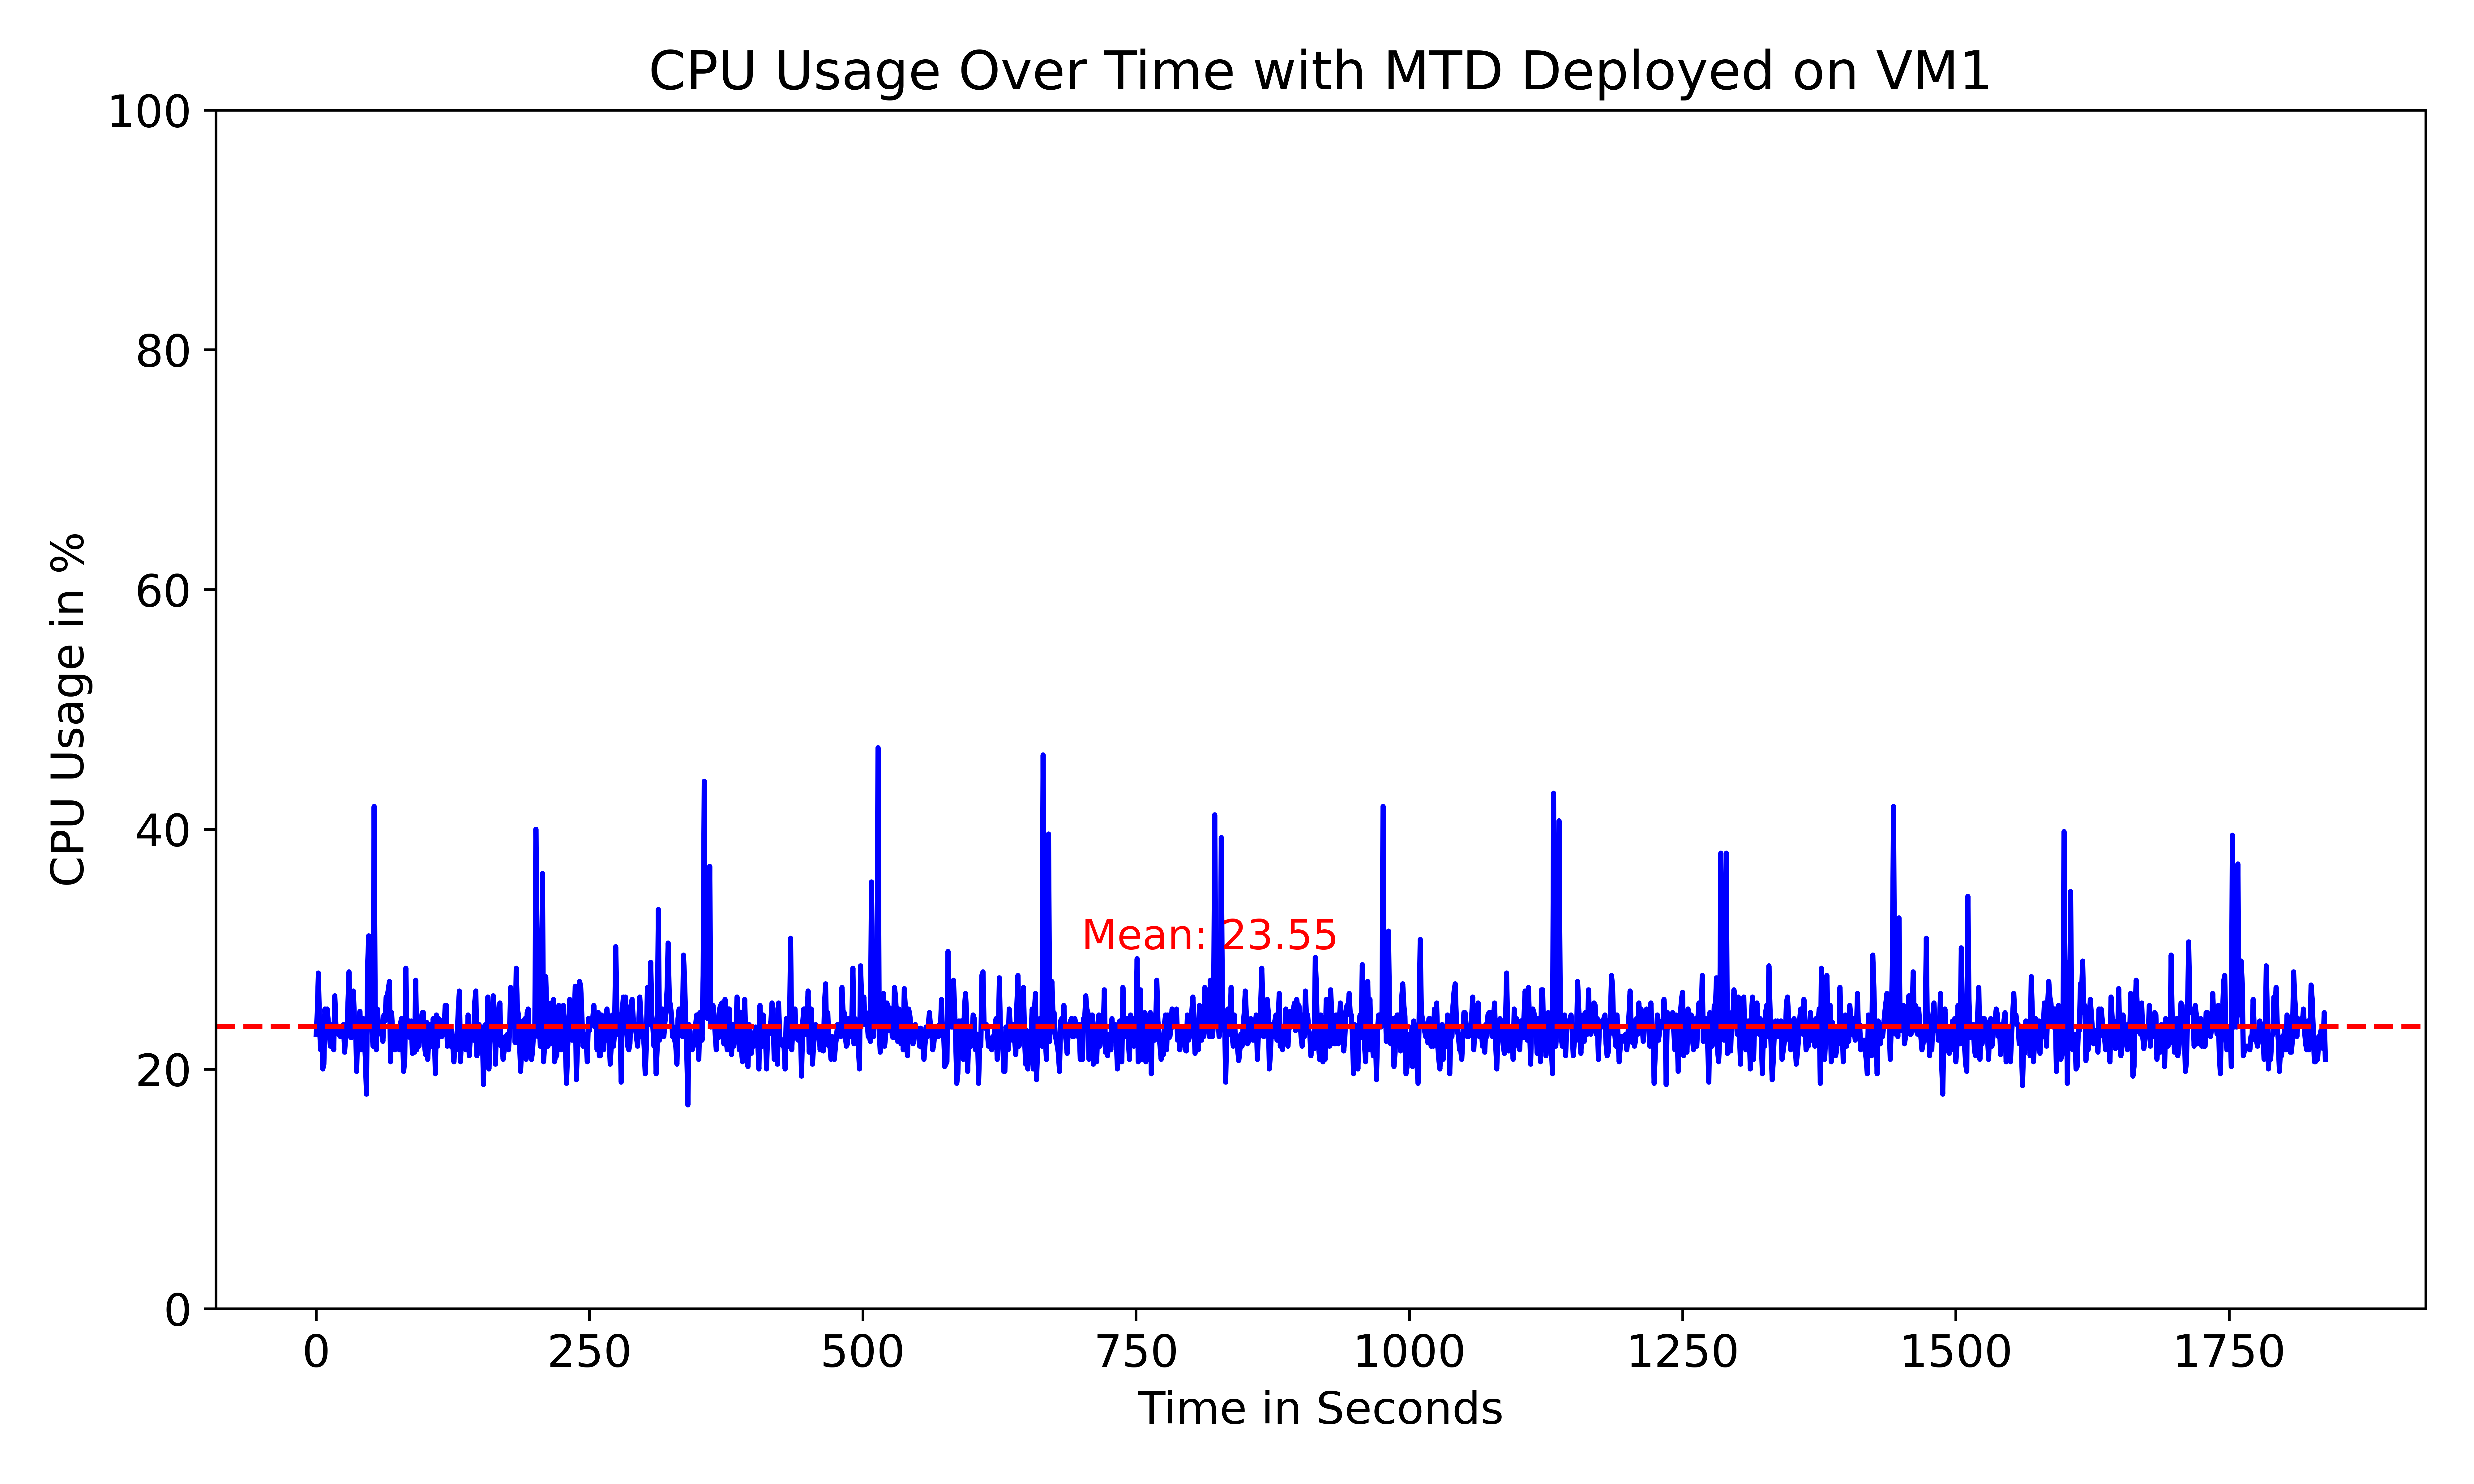
\includegraphics[width=\textwidth]{assets/CPUVM1MTDDeployed.png}
         \caption{The CPU Usage of VM1 With the MTD Mechanism Deployed. This Machine Executed the IP Address Change.}
         \label{graphic:CPUVM1MTDDeployed}
     \end{subfigure}
    \hfill
\end{figure}


\begin{figure}
     \centering
     \begin{subfigure}[b]{0.8\textwidth}
         \centering
         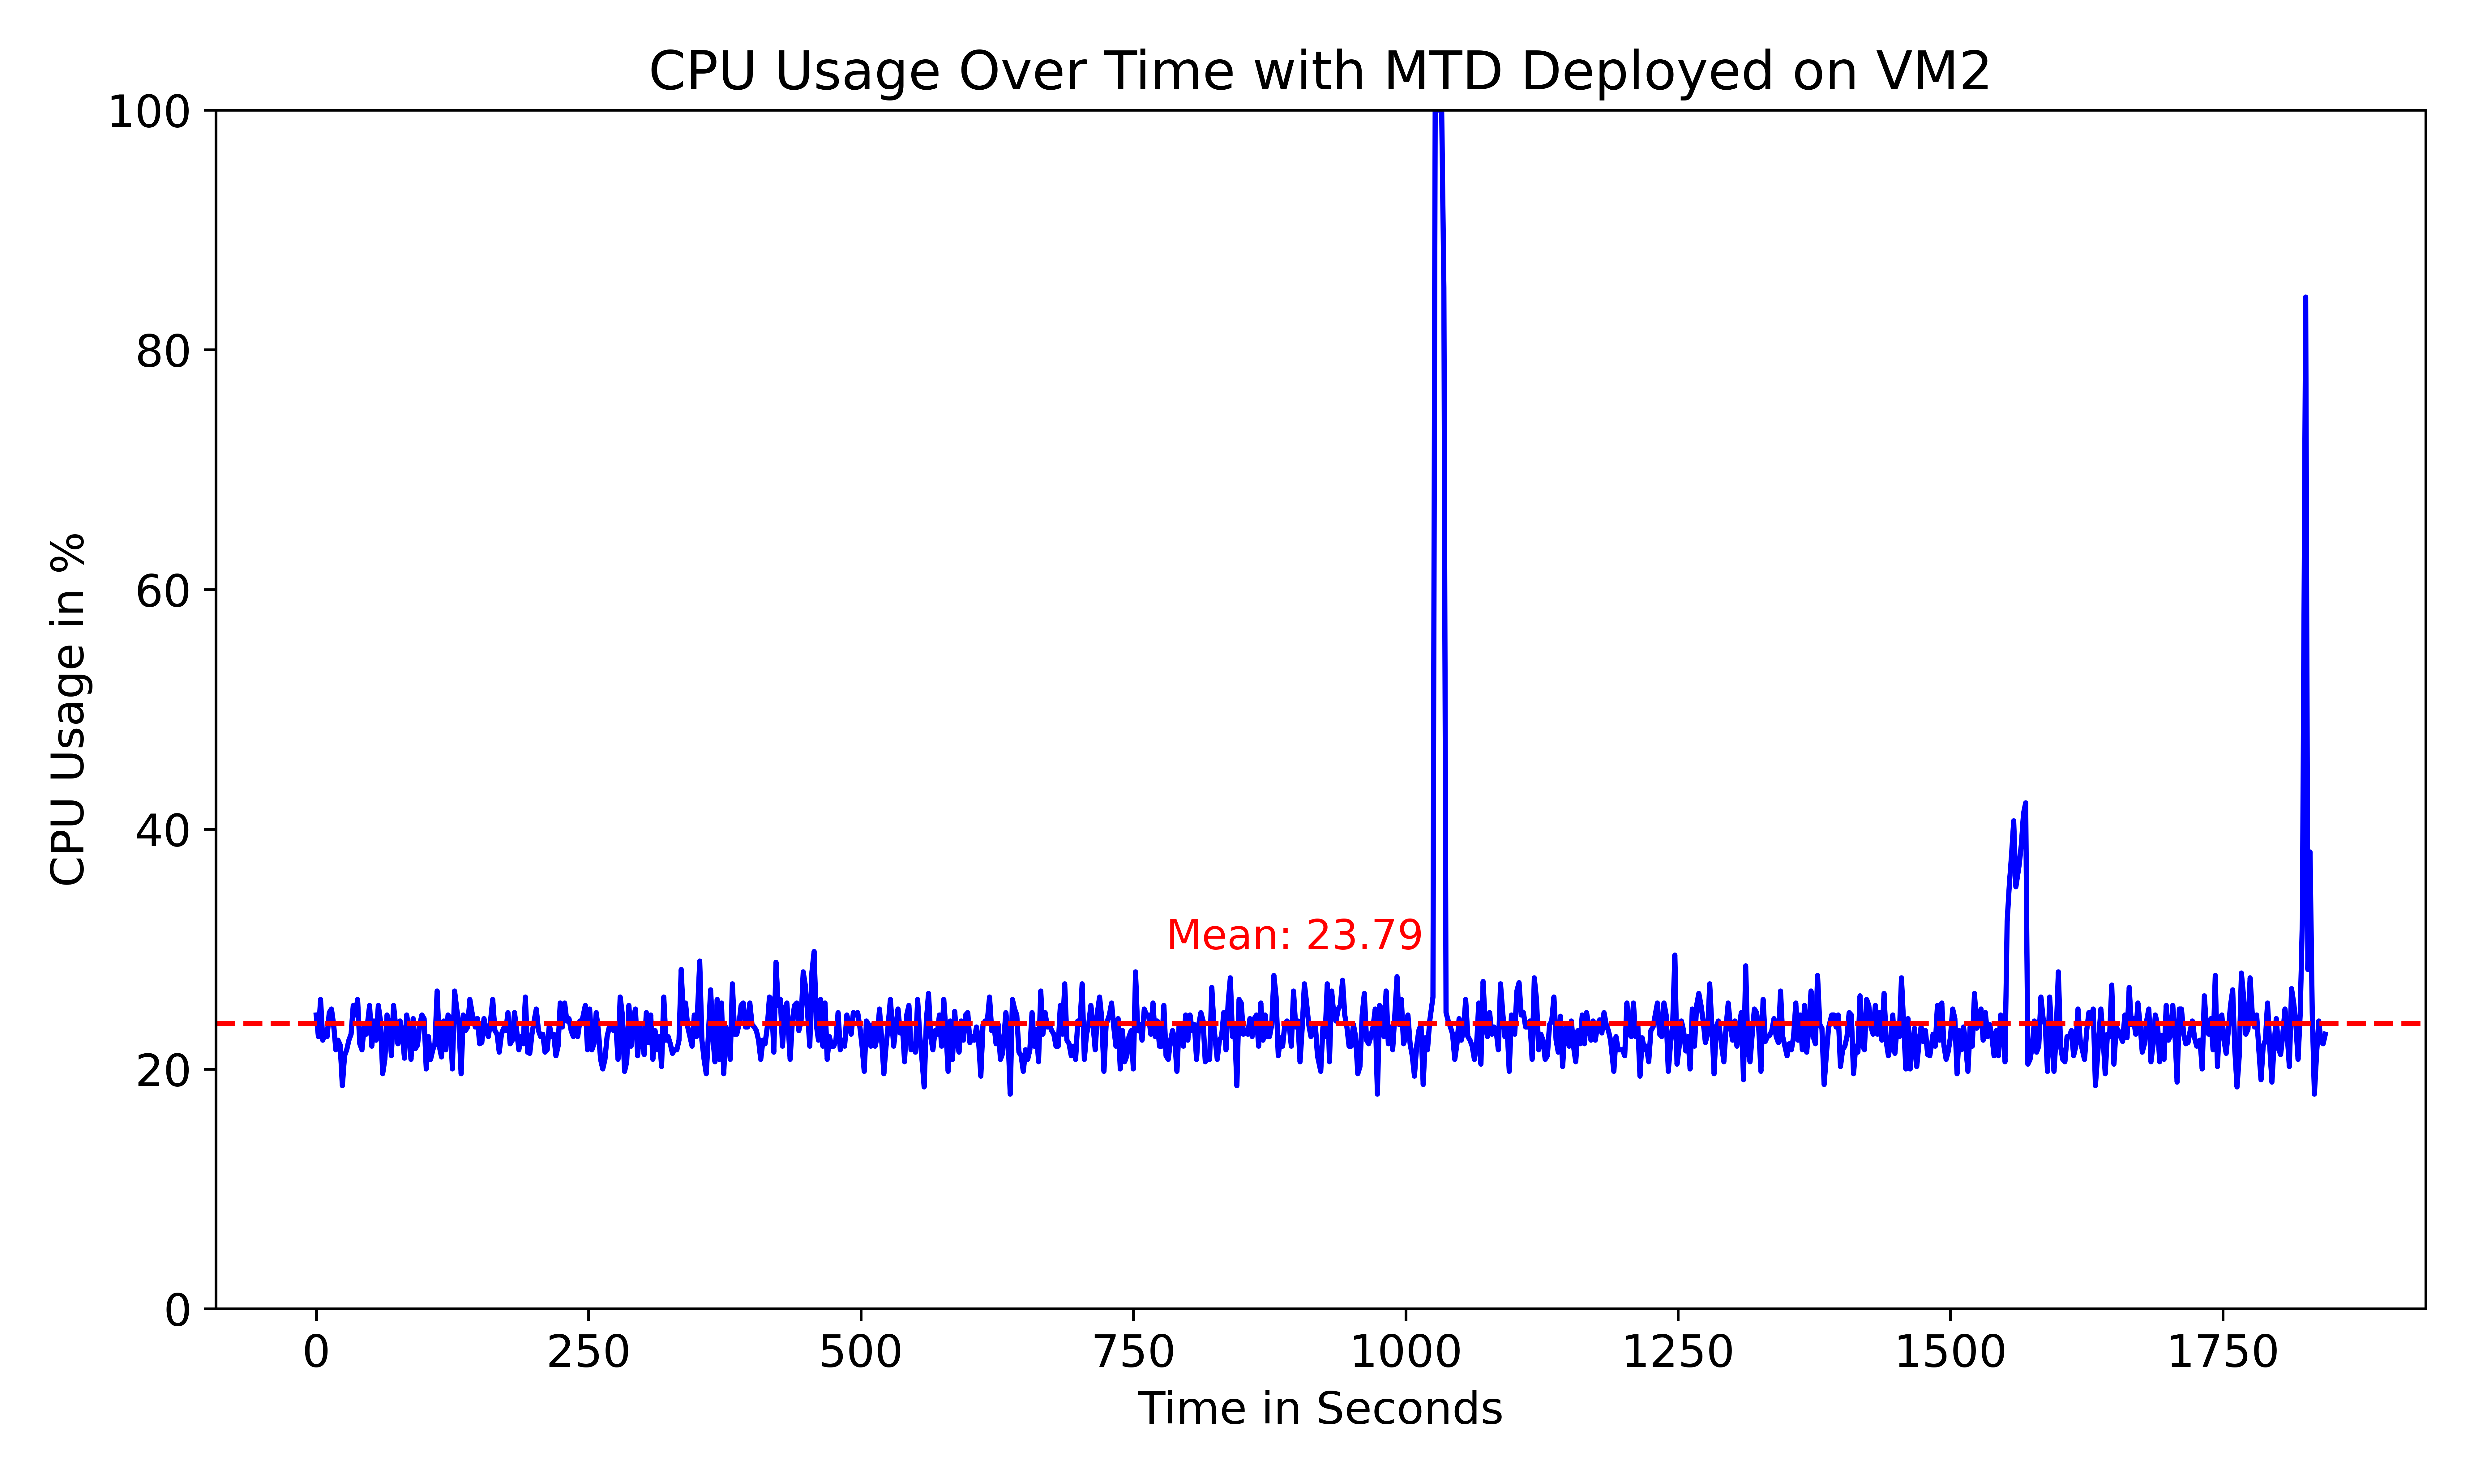
\includegraphics[width=\textwidth]{assets/CPUVM2MTDNotDeployed.png}
         \caption{The CPU Usage of VM2 Without the MTD Mechanism Deployed.}
         \label{graphic:CPUVM2MTDNotDeployed}
     \end{subfigure}
     \hfill
        \begin{subfigure}[b]{0.8\textwidth}
         \centering
         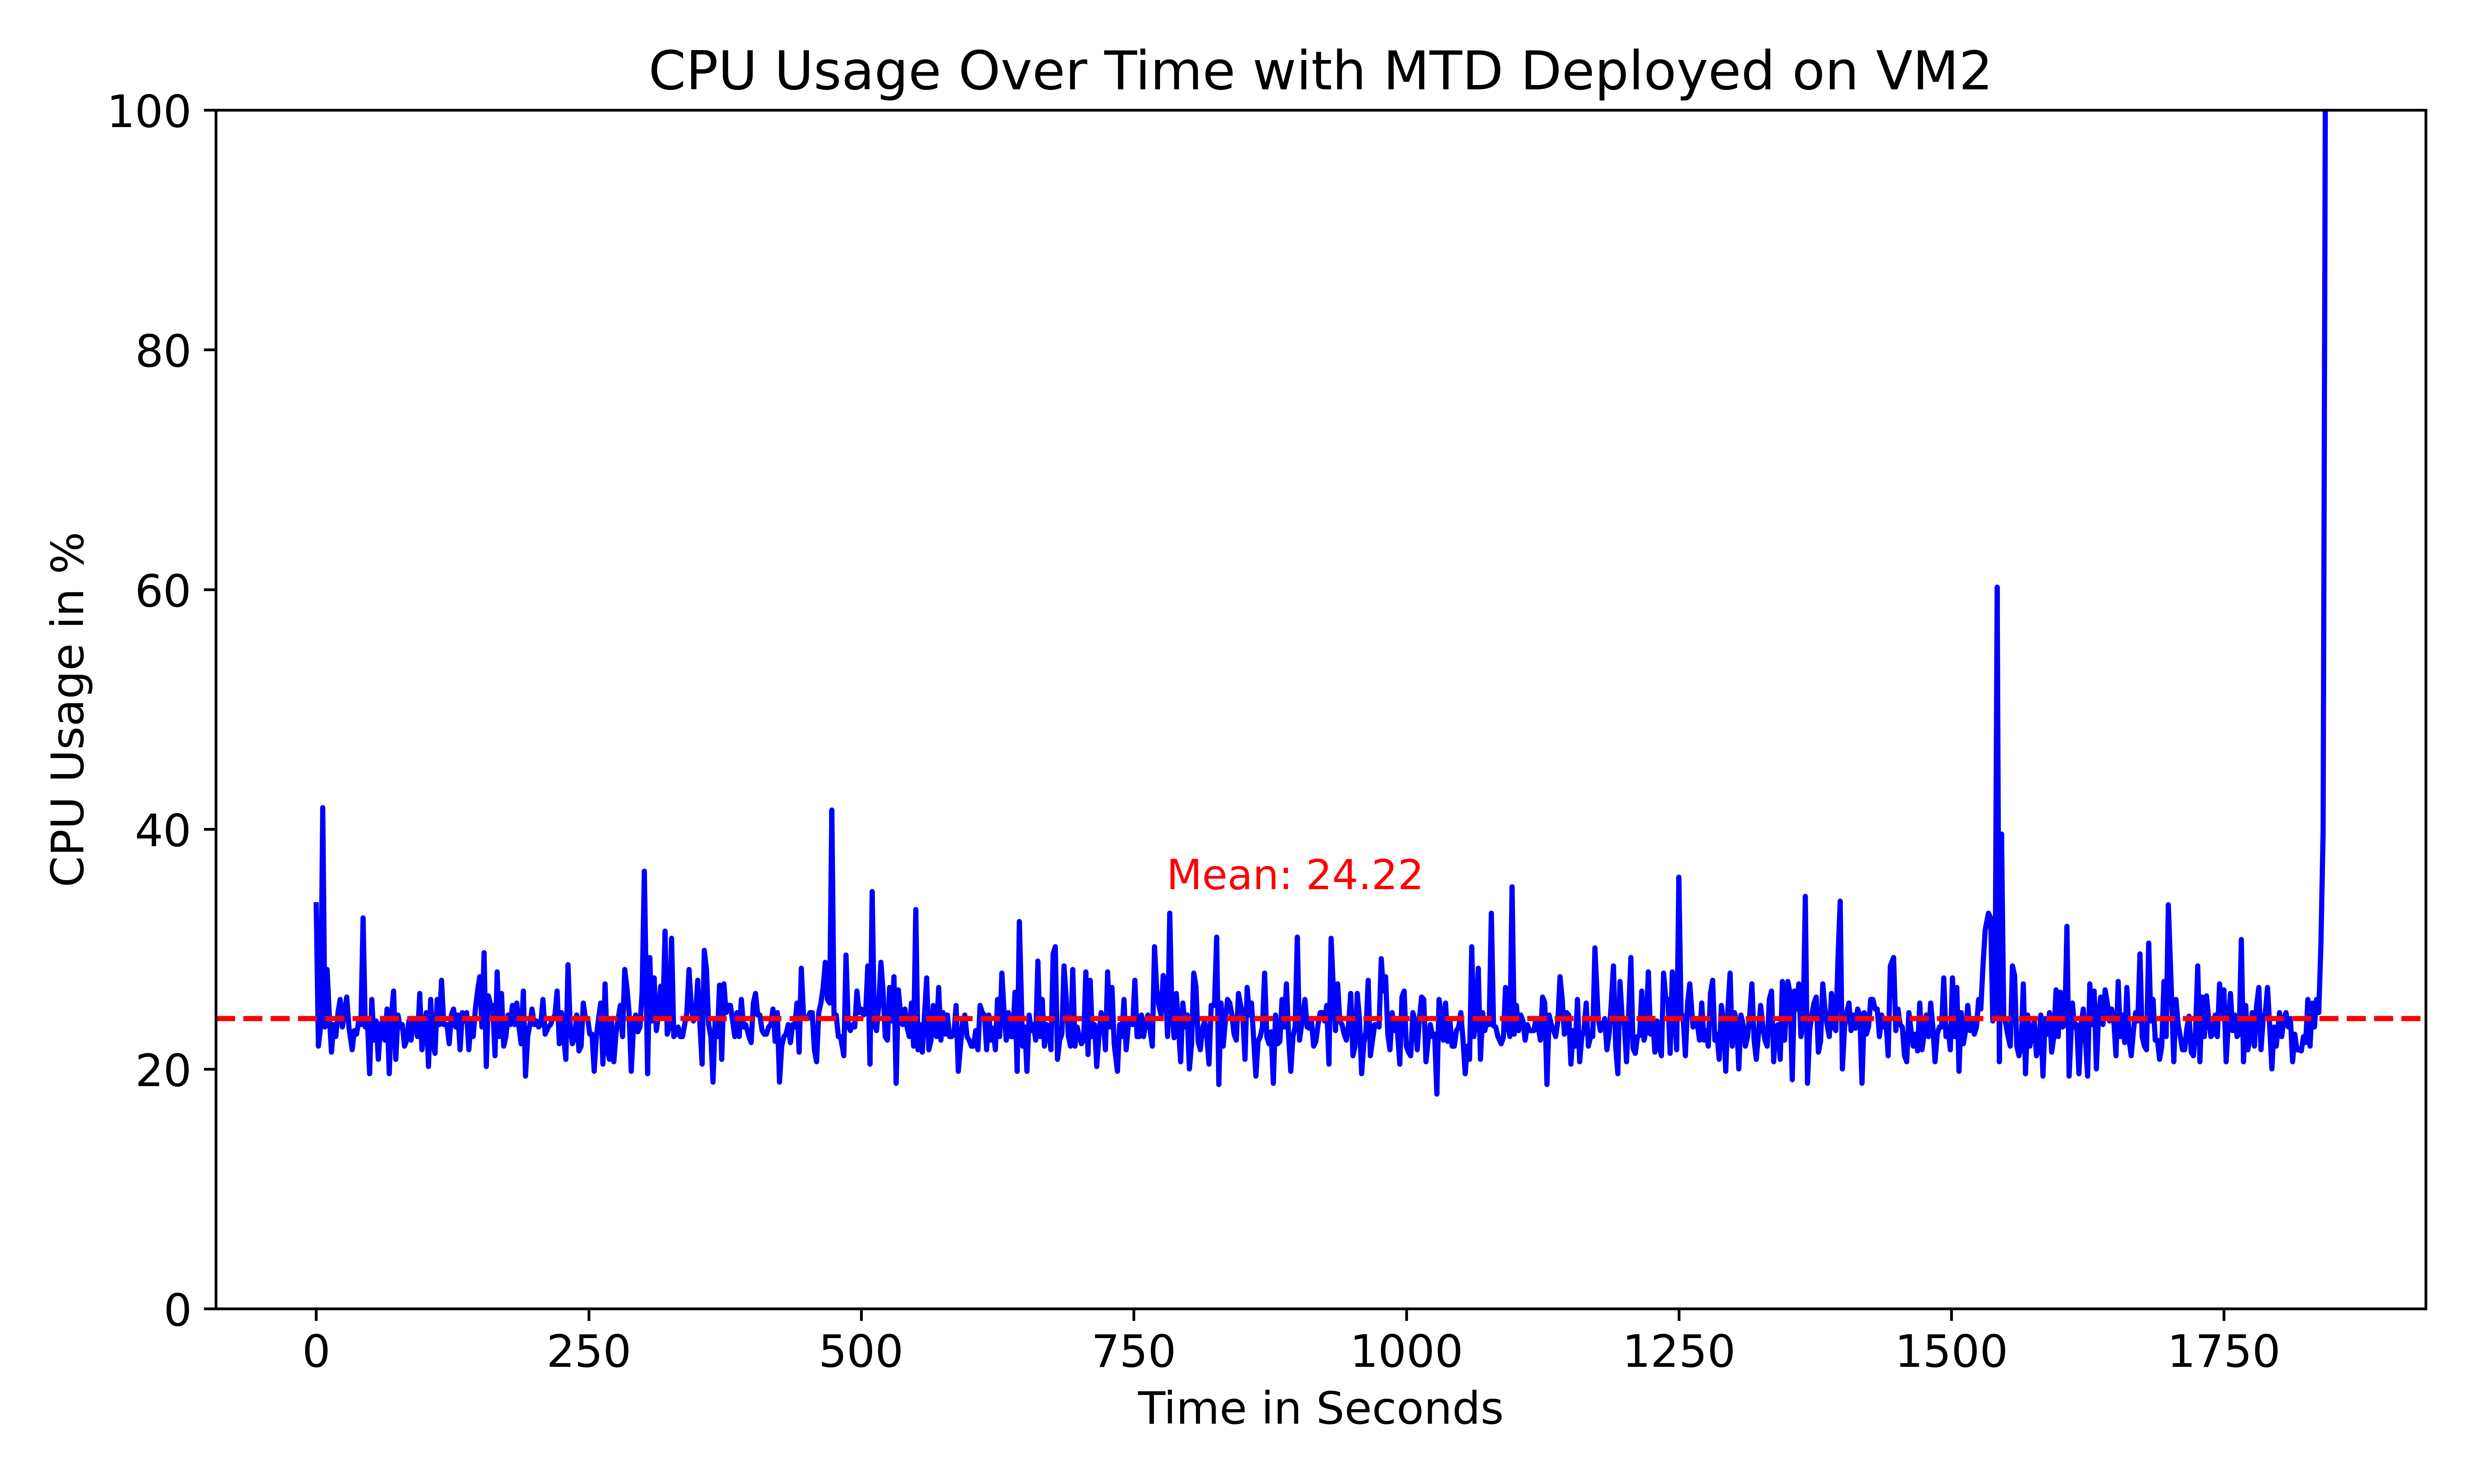
\includegraphics[width=\textwidth]{assets/CPUVM2MTDDeployed.png}
         \caption{The CPU Usage of VM2 With the MTD Mechanism Deployed. This Machine Executed the Telnet Service Port Change.}
         \label{graphic:CPUVM2MTDDeployed}
     \end{subfigure}
     \hfill
\end{figure}


